\documentclass[12pt]{article}
\usepackage{amssymb}
\usepackage{amsmath}
\usepackage{bm}
\usepackage{graphicx}
\usepackage{color, colortbl}
\usepackage{latexsym}
\usepackage{epsfig}
\usepackage{verbatim}
\usepackage{float}
\usepackage[normalem]{ulem}
\usepackage{setspace}
\usepackage{pbox}
\usepackage{color, colortbl}
\definecolor{LightCyan}{rgb}{0.88,1,1}
\usepackage[utf8]{inputenc}
\usepackage[english]{babel}
\setlength{\parskip}{2em}
\renewcommand{\baselinestretch}{1}
\usepackage{geometry}
\geometry{legalpaper, margin=1in}
\usepackage{hyperref}
\hypersetup{
    colorlinks=true,
    linkcolor=blue,
    filecolor=magenta,      
    urlcolor=cyan,
}
 
\urlstyle{same}
%%%%%%%%%%%%%%%%%%%%%%%%%
\author{Aashish Jain}
\title{Springboard Data Science Intensive Capstone Project - Predicting the Likelihood of Flight Cancellations}
\begin{document}
\setcounter{page}{-1}
\maketitle
\thispagestyle{empty}
\thispagestyle{empty}
\newpage
\tableofcontents
\thispagestyle{empty}
\newpage
\large
%%%%%%%%%%%%%%%%%%%%%%%%%
\section{Introduction}
\label{Sec:intro}
%%%%%%%%%%%%%%%%%%%%%%%%%
Imagine you have a trip coming up in next few days and someone tells you that ``your flight has a high chance of being canceled, so be aware of that and rethink about your travel, hotel bookings, etc..". That would be helpful for you and all other passengers traveling out there. Even though the flight cancellation rate is not high (about 1-2$\%$ in the US domestic market), that one rare event causes a lot of troubles to passengers in terms of rescheduling their travel plans. There are many factors such as flight date and time, origin and destination airport, airline type, weather, etc.. which might affect the cancellation rate. We use data from various sources containing these factors and propose to build a machine learning model for predicting the likelihood of flight cancellation for US domestic flights operating at selected airports.


Travel planners and booking companies such as booking.com, expedia.com, kayak.com, priceline.com, etc. can use such a model to predict the likelihood of the cancellation of a flight. They can then inform their customers well in advance, even before the airlines' management informs the passengers, about the probability of the cancellation of their upcoming flight. From the traveler's point of view, it would be very convenient for them. On the other hand, such a predictive model would enhance the product base of travel planner companies. Moreover, there is a possibility of developing an app which travelers can use to know about their flight cancellation likelihood in advance.
%%%%%%%%%%%%%%%%%%%%%%%%%
\section{Data Acquisition and Cleaning}
\label{sec:dataclean}
%%%%%%%%%%%%%%%%%%%%%%%%%
We acquire datasets from two different sources. The first dataset contains flight information and the second dataset has information about the weather. 


The flight data is acquired from the \href{https://www.transtats.bts.gov/DL_SelectFields.asp?Table_ID=236&DB_Short_Name=On-Time}{Bureau of Transportation Statistics}. This website allows downloading data for one month at a time. We downloaded data for multiple months and concatenated all the data together. More details about acquiring and concatenating the data can be found in \href{https://github.com/aajains/springboard-datascience-intensive/blob/master/capstone_project/DataAcquisitionMerging/data_acquisition_merging.ipynb}{this IPython notebook}. Each row in the flight dataset corresponds to a unique flight with details such as flight date, carrier name, origin airport, destination airport, departure time, arrival time, distance, departure delay, arrival delay, cancellation status, taxi times, and many other on-performance data. We have also extracted some historical information about the flights and added new columns. The historical data contains information about flight delays, cancellation, diversions, etc.. in last ``ndays" with three values of ``ndays = 10, 20, 30". More details about the calculations of historical performance can be found in \href{https://github.com/aajains/springboard-datascience-intensive/blob/master/capstone_project/DataAcquisitionMerging/history_calc.ipynb}{this IPython notebook}.


The hourly weather data is downloaded using \href{https://www.wunderground.com/weather/api}{wunderground.com API} in XML format. The weather data contains information such as temperature, humidity, visibility, wind direction, weather condition etc.. One API call can be used to download data for a chosen airport and a chosen date (for all hours on that date). So, if we want to get the weather data for one airport, say LAX, for two years, we would need close to $2 \times 365 = 730$ API calls. Due to some restrictions on number of API calls per day and also on API call rate (per minute), we acquired data for only top 20 airports (in terms of observing the most traffic during 2015-2016). More details about accessing the weather data and parsing it to a proper format can be found in \href{https://github.com/aajains/springboard-datascience-intensive/blob/master/capstone_project/DataAcquisitionMerging/weather.ipynb}{this IPython notebook}.

Having the two datasets, we then merge them such that we get the weather information for each flight at its origin and destination locations. More details on merging these datasets can be found in \href{https://github.com/aajains/springboard-datascience-intensive/blob/master/capstone_project/DataAcquisitionMerging/data_acquisition_merging.ipynb}{this IPython notebook}. Other than having missing values already in the original datasets, merging the datasets also generates some missing values. We fix all the missing values by either imputations or by filling them with zeros. We also remove some of the columns that do not provide any meaningful information. More details on the data cleaning process can be found in \href{https://github.com/aajains/springboard-datascience-intensive/blob/master/capstone_project/DataCleaning/data_cleaning.ipynb}{this IPython notebook}. The cleaned dataset is then ready for explorations.
%%%%%%%%%%%%%%%%%%%%%%%%%
\section{Data Exploration}
\label{sec:eda}
%%%%%%%%%%%%%%%%%%%%%%%%%
%%%%%%%%%%%%%%%%%%%%%%%%%
\subsection{Introduction to the cleaned data}
\label{subsec:dataintro}
%%%%%%%%%%%%%%%%%%%%%%%%%
There are 1,417,308 and 1,439,831 records for years 2015 and 2016, respectively, and 90 fields. In this project, we considered top 20 airports in the US (in terms of most traffic). These 20 airports network broadly covers the whole US as shown in Fig. \ref{fig:map}. 
\begin{figure}[h!]
\begin{center}
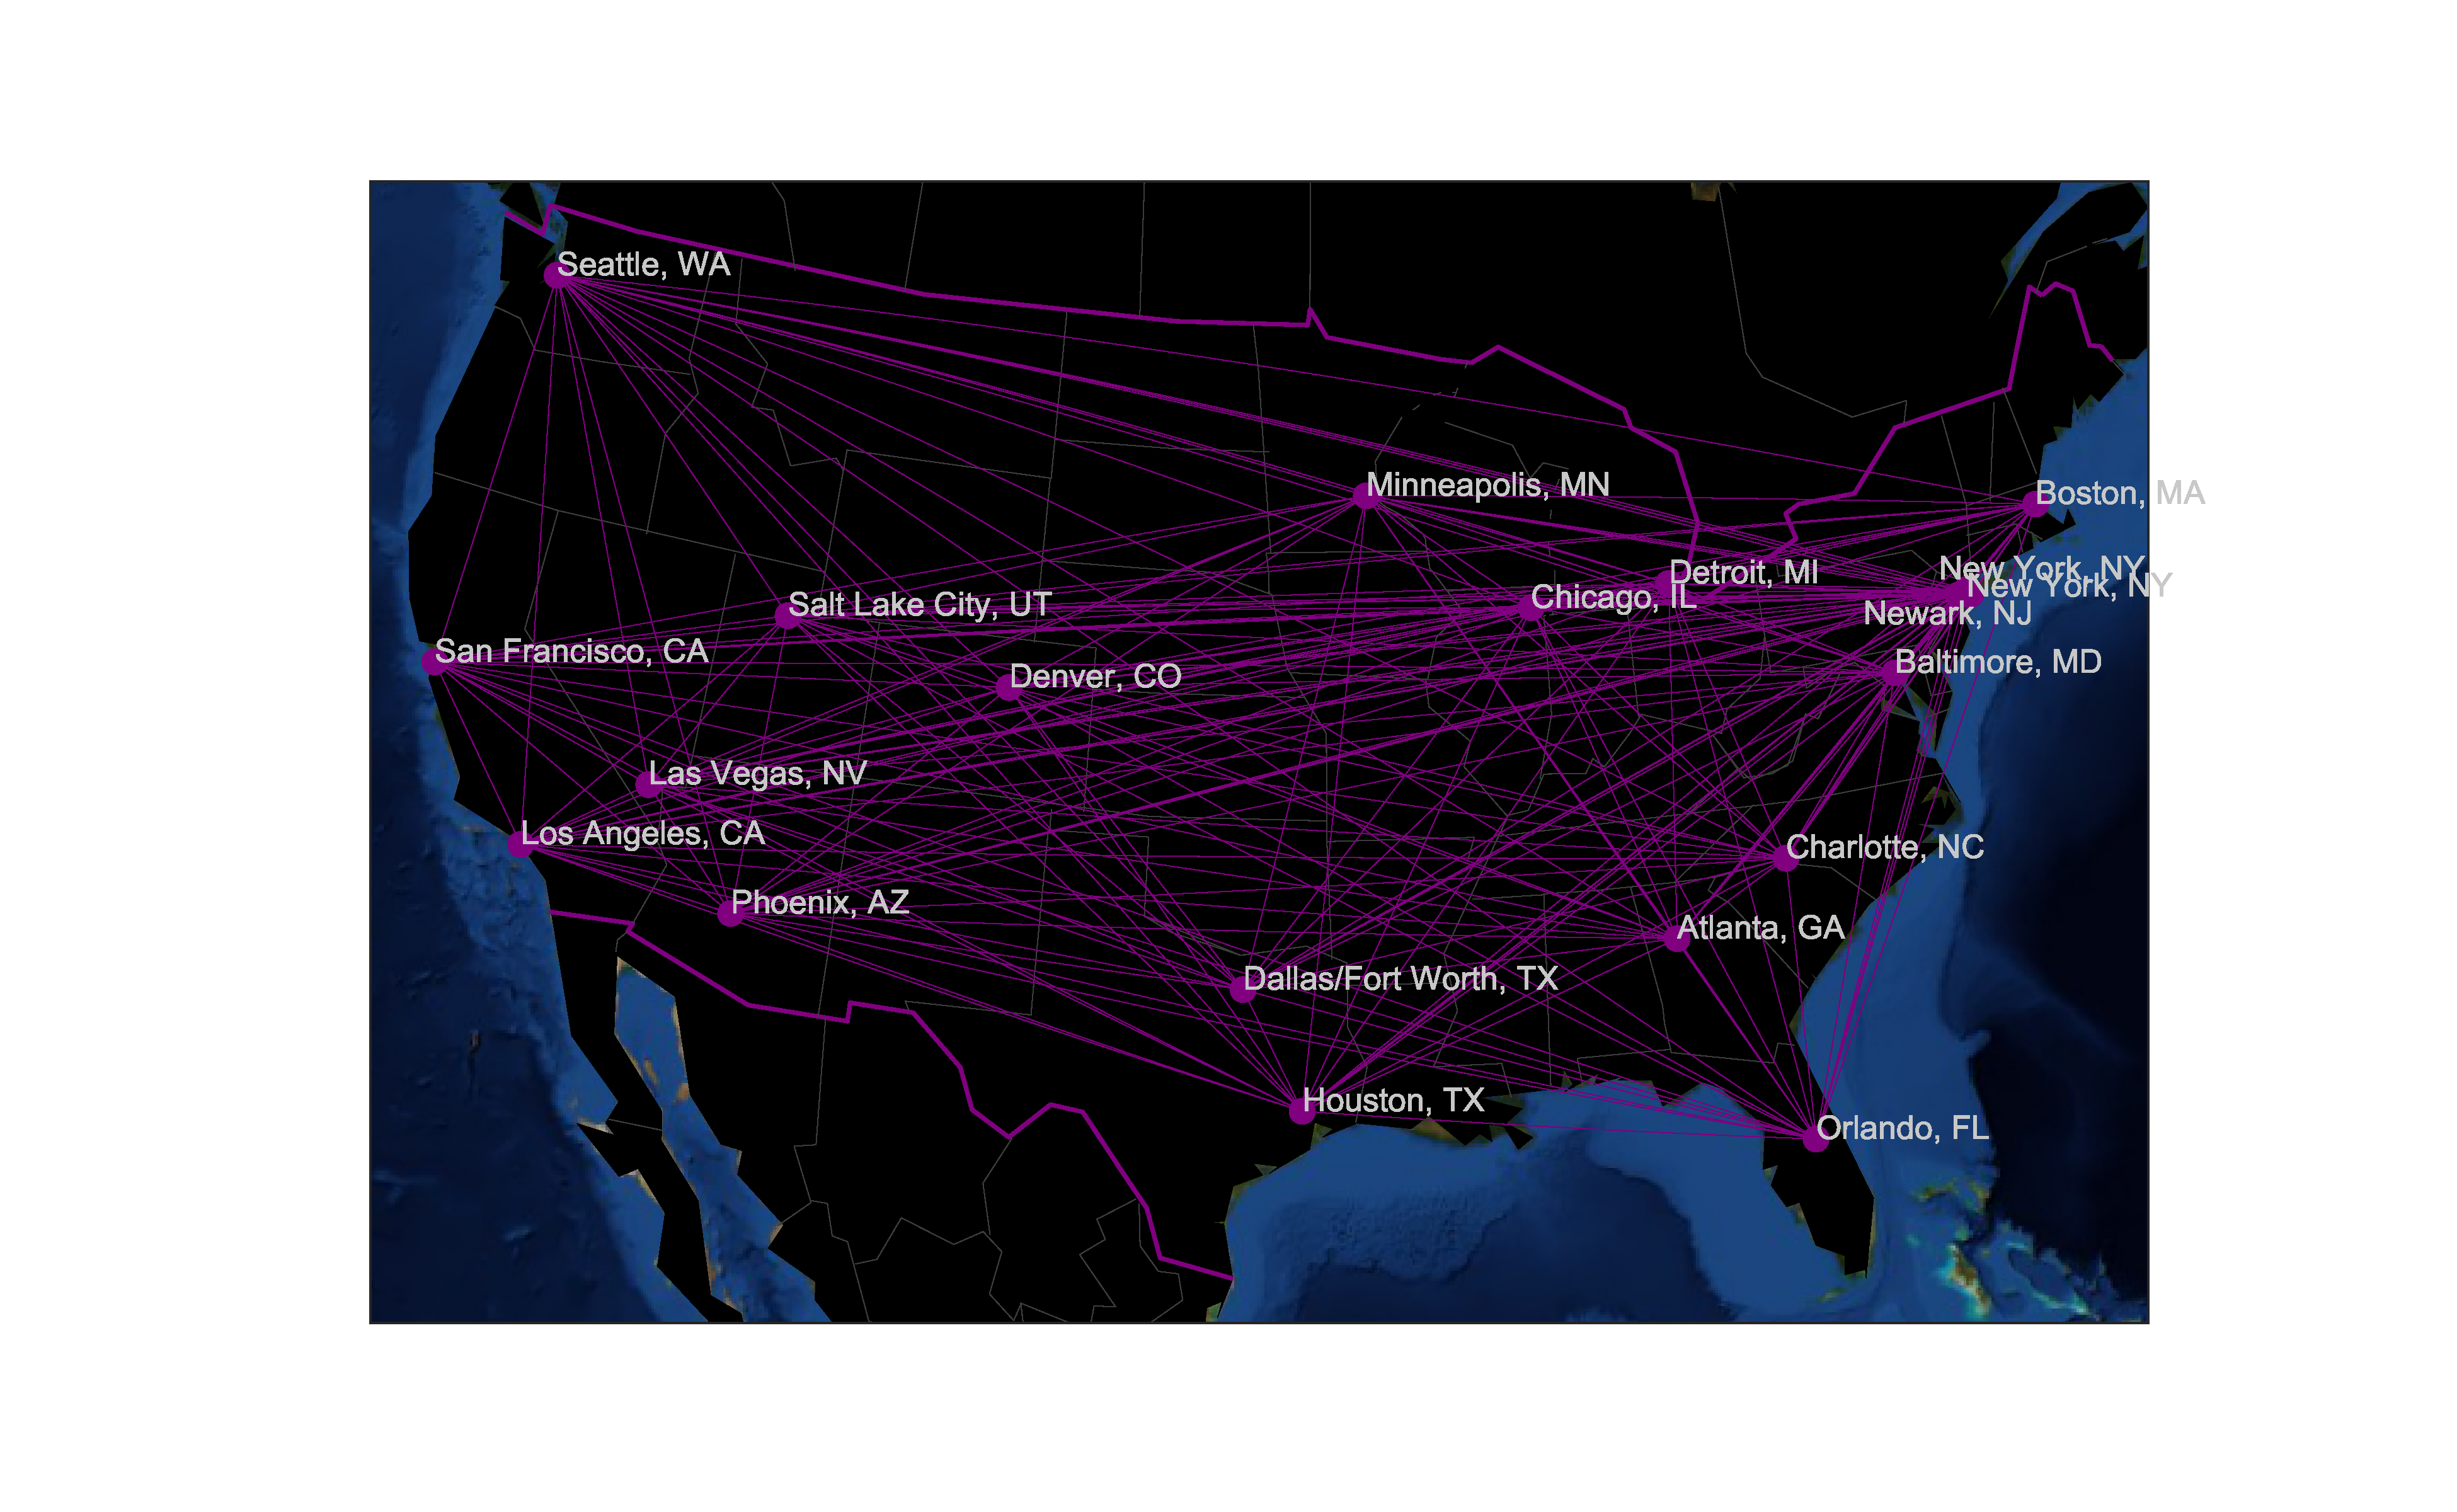
\includegraphics[width=6in]{map.pdf}
\end{center}
\caption{\label{fig:map}
Network of top 20 airports in the US. Note that there are two airports in the New York City: LGA and JFK.}
\end{figure}
The justification for selecting these 20 airports is discussed in detail in \href{https://github.com/aajains/springboard-datascience-intensive/blob/master/capstone_project/DataAcquisitionMerging/data_acquisition_merging.ipynb}{this IPython notebook}. 


We will go through most of the fields (or columns) in the dataset to explore their relationship with flight cancellation rate. Details about each field can be found in \href{https://www.transtats.bts.gov/Fields.asp?Table_ID=236}{the Bureau of Transportation Statistics} and \href{https://www.wunderground.com/weather/api/d/docs?d=resources/phrase-glossary}{the Wunderground} websites and some in \href{https://github.com/aajains/springboard-datascience-intensive/blob/master/capstone_project/DataAcquisitionMerging/history_calc.ipynb}{this IPython notebook} and \href{https://github.com/aajains/springboard-datascience-intensive/blob/master/capstone_project/DataCleaning/data_cleaning.ipynb}{this IPython notebook}. The target column for this project is called  "Cancelled" which contains two values: 1 for cancelled flights and 0 for not-cancelled flights. 
%%%%%%%%%%%%%%%%%%%%%%%%%
\subsection{Flight Cancellation Rate}
\label{subsec:canrate}
%%%%%%%%%%%%%%%%%%%%%%%%%
Out of 2.8$+$ million flights operating at top 20 airports in 2015-2016, about 1.15$\%$ of them got cancelled. This does not seem like a large number but such rare events cause a great deal of inconveniences to passengers, and cost a lot of money to airline companies. Therefore, it is important to understand where, when and how this small events occur. To start with, we plot the total number of flights on a daily basis and see how many flights got cancelled (on a daily basis) in Fig. \ref{fig:daily}. 
\begin{figure}[h!]
\begin{center}
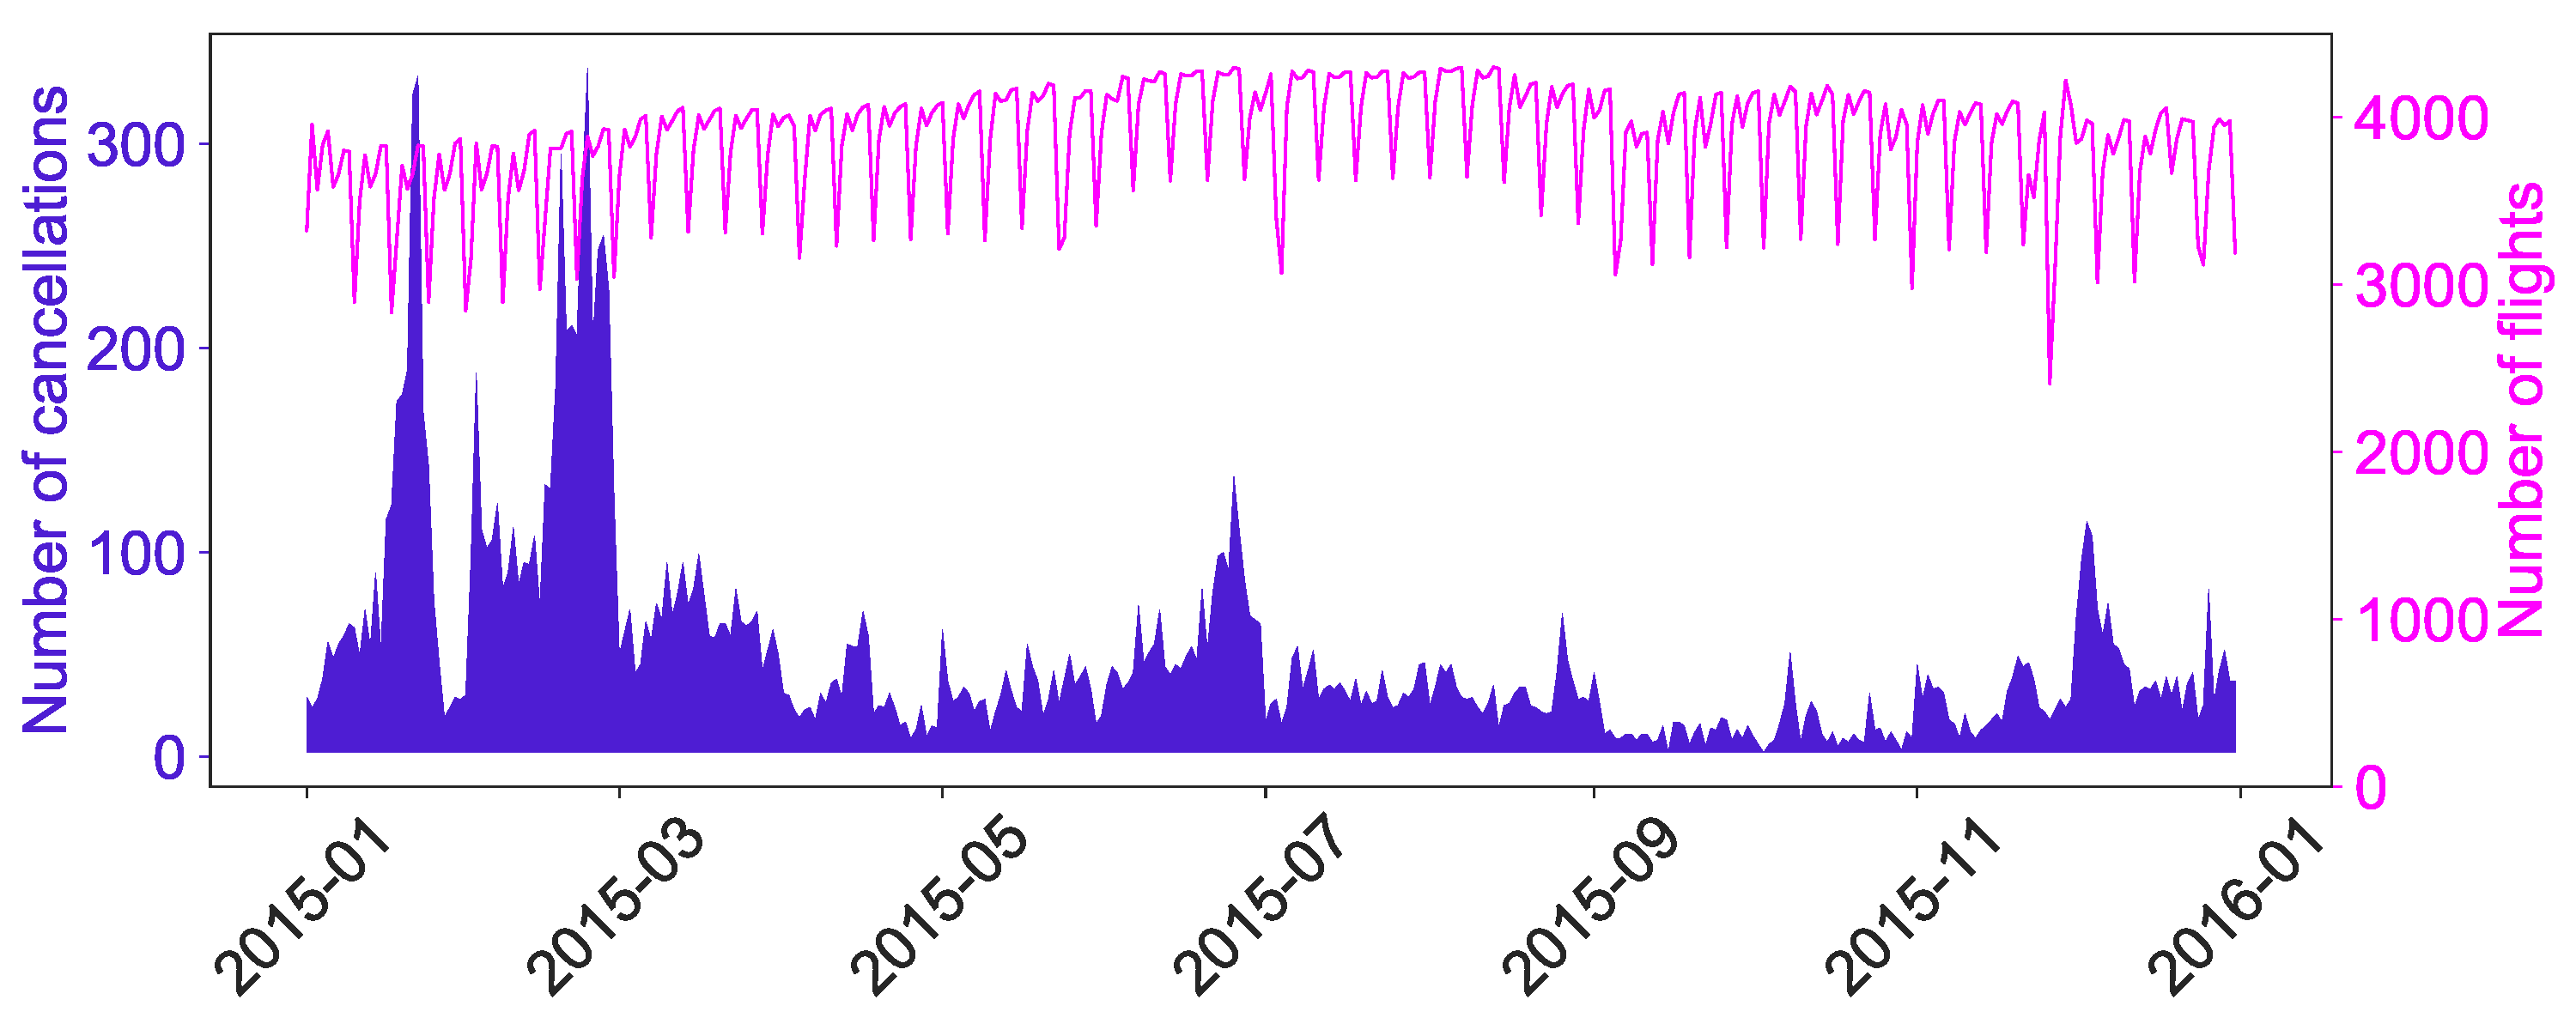
\includegraphics[width=6in]{daily_flights_cancellations.pdf}
\end{center}
\caption{\label{fig:daily}
Total number of flights (right y-axis) and number of cancelled flights (left y-axis), on a daily basis.}
\end{figure}
The daily total number of flights remain almost steady with regular and periodic troughs. The number of cancelled flights has no steady trend but has some big spikes. Knowing the number of flights and number of cancellations, we can calculate the cancellation rate for a given day. We define the cancellation rate as, 
\begin{equation}
\label{eq:canrate}
\text{Flight cancellation rate} = \frac{\text{Number of flights cancelled for a given scenario}}{\text{Total number of flights for a given scenario}},
\end{equation}
where a ``scenario" can refer to a class of a field. In the plot above, a scenario would refer to a date, say June 24th 2015. Figure \ref{fig:dailycanrate} shows the daily $\%$ cancellation rates.  
\begin{figure}[h!]
\begin{center}
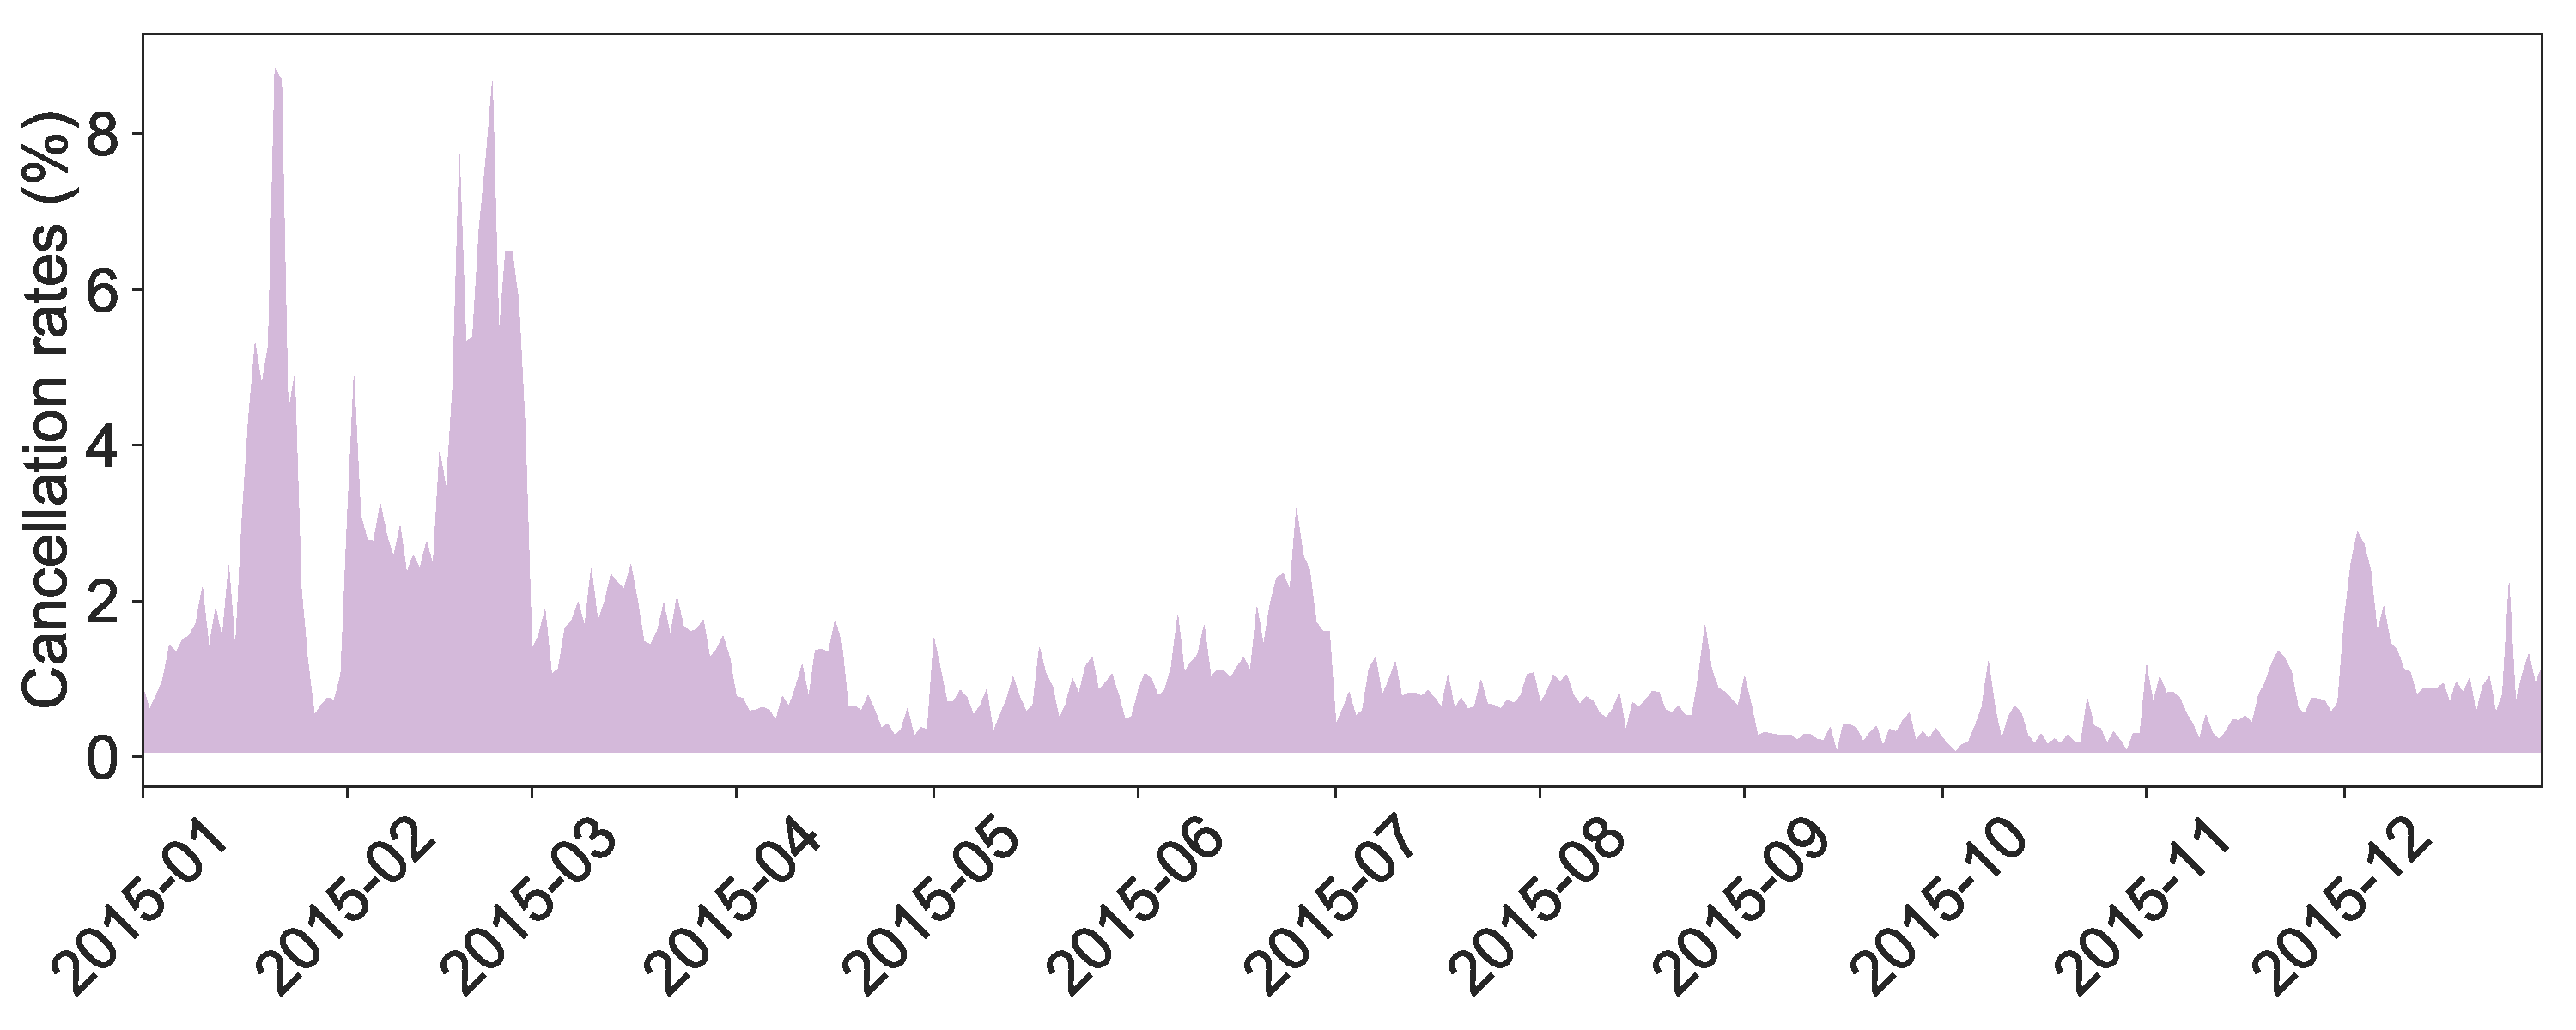
\includegraphics[width=6in]{daily_canrate.pdf}
\end{center}
\caption{\label{fig:dailycanrate}
Daily cancellation rates.}
\end{figure}
Big spikes in the cancellation rates were mainly caused by bad weather as depicted above. There were some spikes in cancellation activities in the end of June and beginning of December too.


We can discuss some other examples for cancellation rates also. For instance, if the field is weather condition which has classes such as Heavy Snow, Rain, Clear Sky etc.., a scenario can be one of these weather conditions. We then count the number of flights operating under such a scenario (say Heavy Snow) and also count the number of flights that got cancelled under the same scenario. Equation~(\ref{eq:canrate}) can then be used to calculate the cancellation rate when the weather condition is Heavy Snow. In the following few sub-sections, we will go through many interesting fields and explore the trend for cancellation rates. There are broadly 6 categories of information that are embedded in all the fields: 
\begin{enumerate}
\itemsep0em
\item Calendar variables
\item Airports
\item Airlines
\item Flight distance
\item Weather factors
\item Historical performances 
\end{enumerate}
%%%%%%%%%%%%%%%%%%%%%%%%%
\subsection{Calendar Variables}
\label{subsec:calvar}
%%%%%%%%%%%%%%%%%%%%%%%%%
There are many calendar variables such as quarter, month, week, day, hour, minute, etc.. Here, we explore the dependency of cancellation rates on month, day of week and scheduled hour. For some flights the origin and destination calendar variables can be different, and hence we calculate the cancellation rates for all variables at both origin and destination airports. Figure \ref{fig:monthlycanrate} shows the monthly cancellation rate.  
\begin{figure}[h!]
\begin{center}
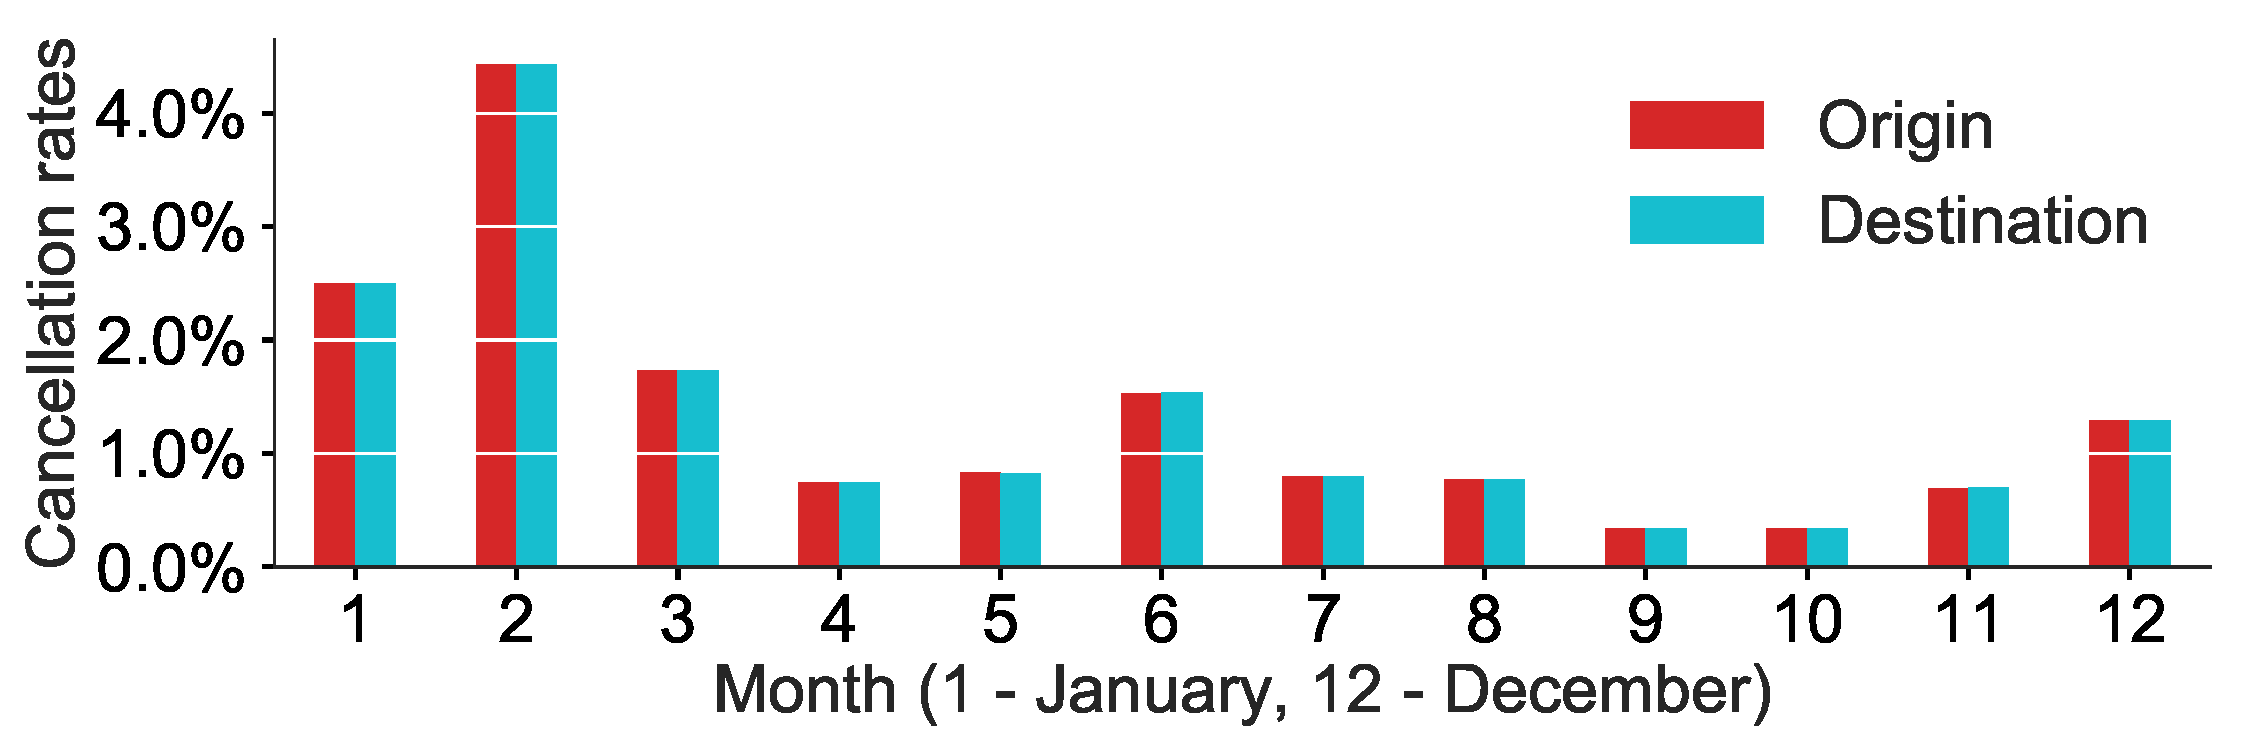
\includegraphics[width=6in]{monthly_canrate.pdf}
\end{center}
\caption{\label{fig:monthlycanrate}
Monthly cancellation rates.}
\end{figure}
There is no difference in cancellation rates between the origin and the destination airports in any given month. February was the worst followed by January and March. We see some mild spikes for June and December too. The high cancellation rate in January and February was mainly due to the snow storms in the east coast. We can also look at the day of the week and understand its influence on the cancellation rate in Fig. \ref{fig:weeklycanrate}. 
\begin{figure}[h!]
\begin{center}
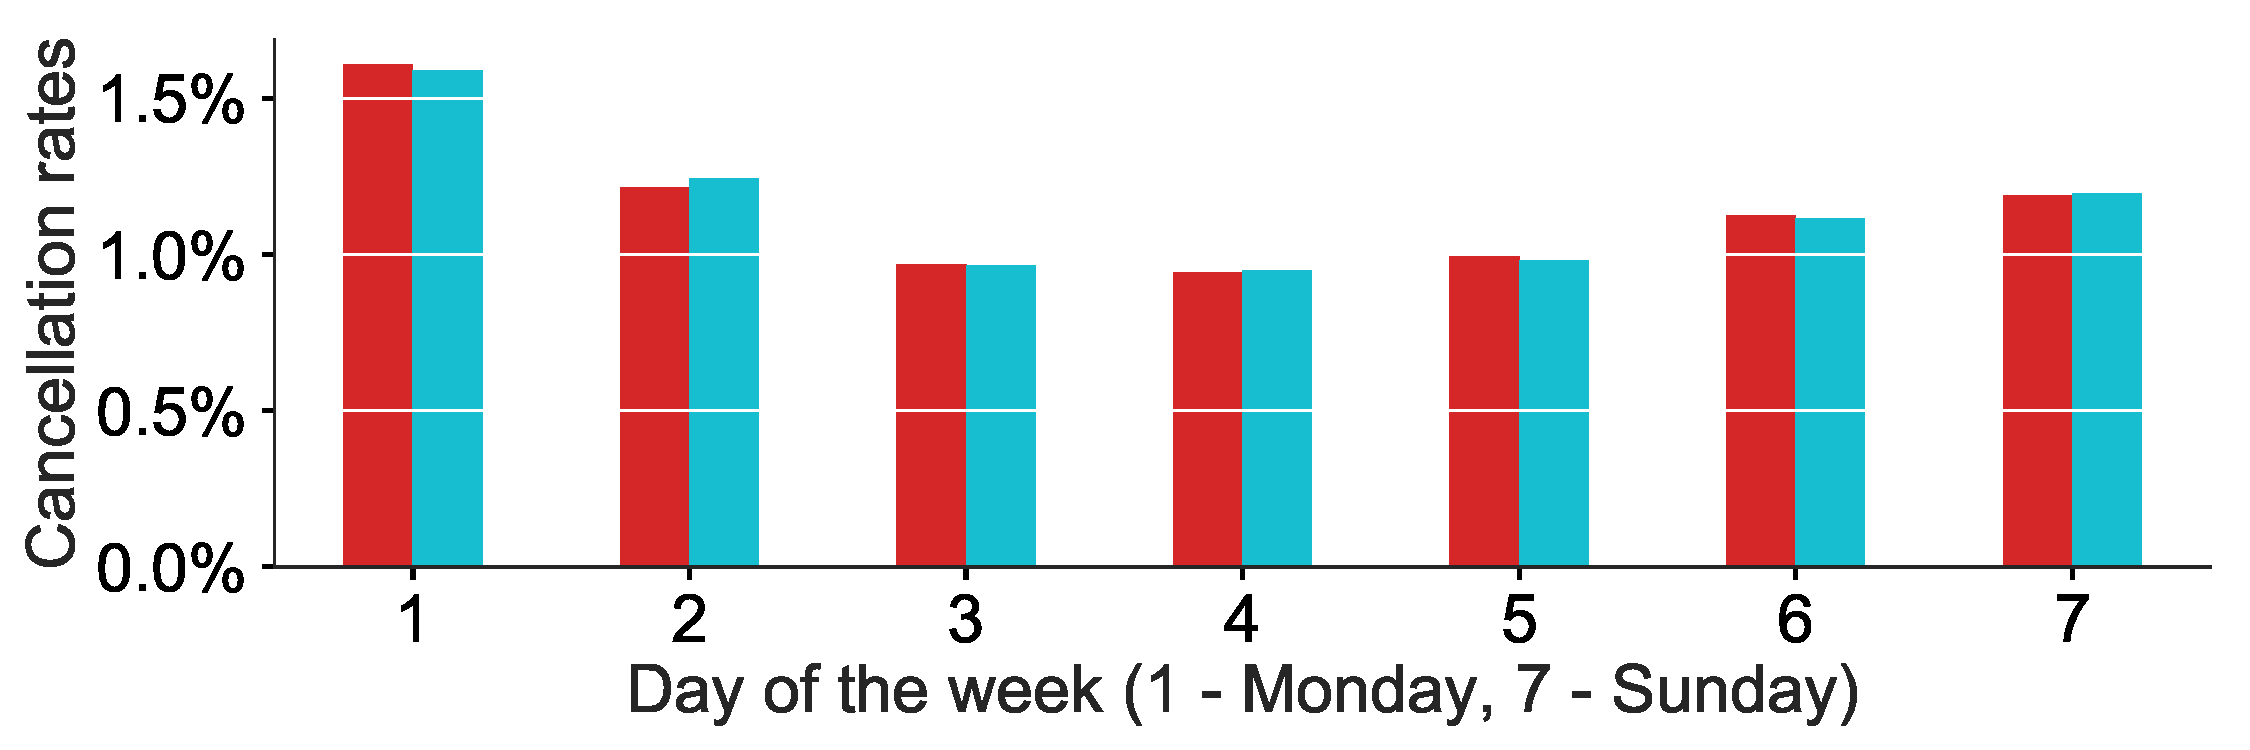
\includegraphics[width=6in]{weekly_canrate.pdf}
\end{center}
\caption{\label{fig:weeklycanrate}
Cancellation rates depend on the day of the week. Note the colors correspond to the same legend as in Fig.\ref{fig:monthlycanrate}.}
\end{figure}
End of the weekend and beginning of the week observed higher cancellation rates as compared to the middle week days. There are very slight differences in cancellation rates between the origin and the destination airports for any day of the week. We can go down one more level in the calendar variable space and explore the hours of the flights throughout the day in Fig. \ref{fig:hourlycanrate}.
\begin{figure}[h!]
\begin{center}
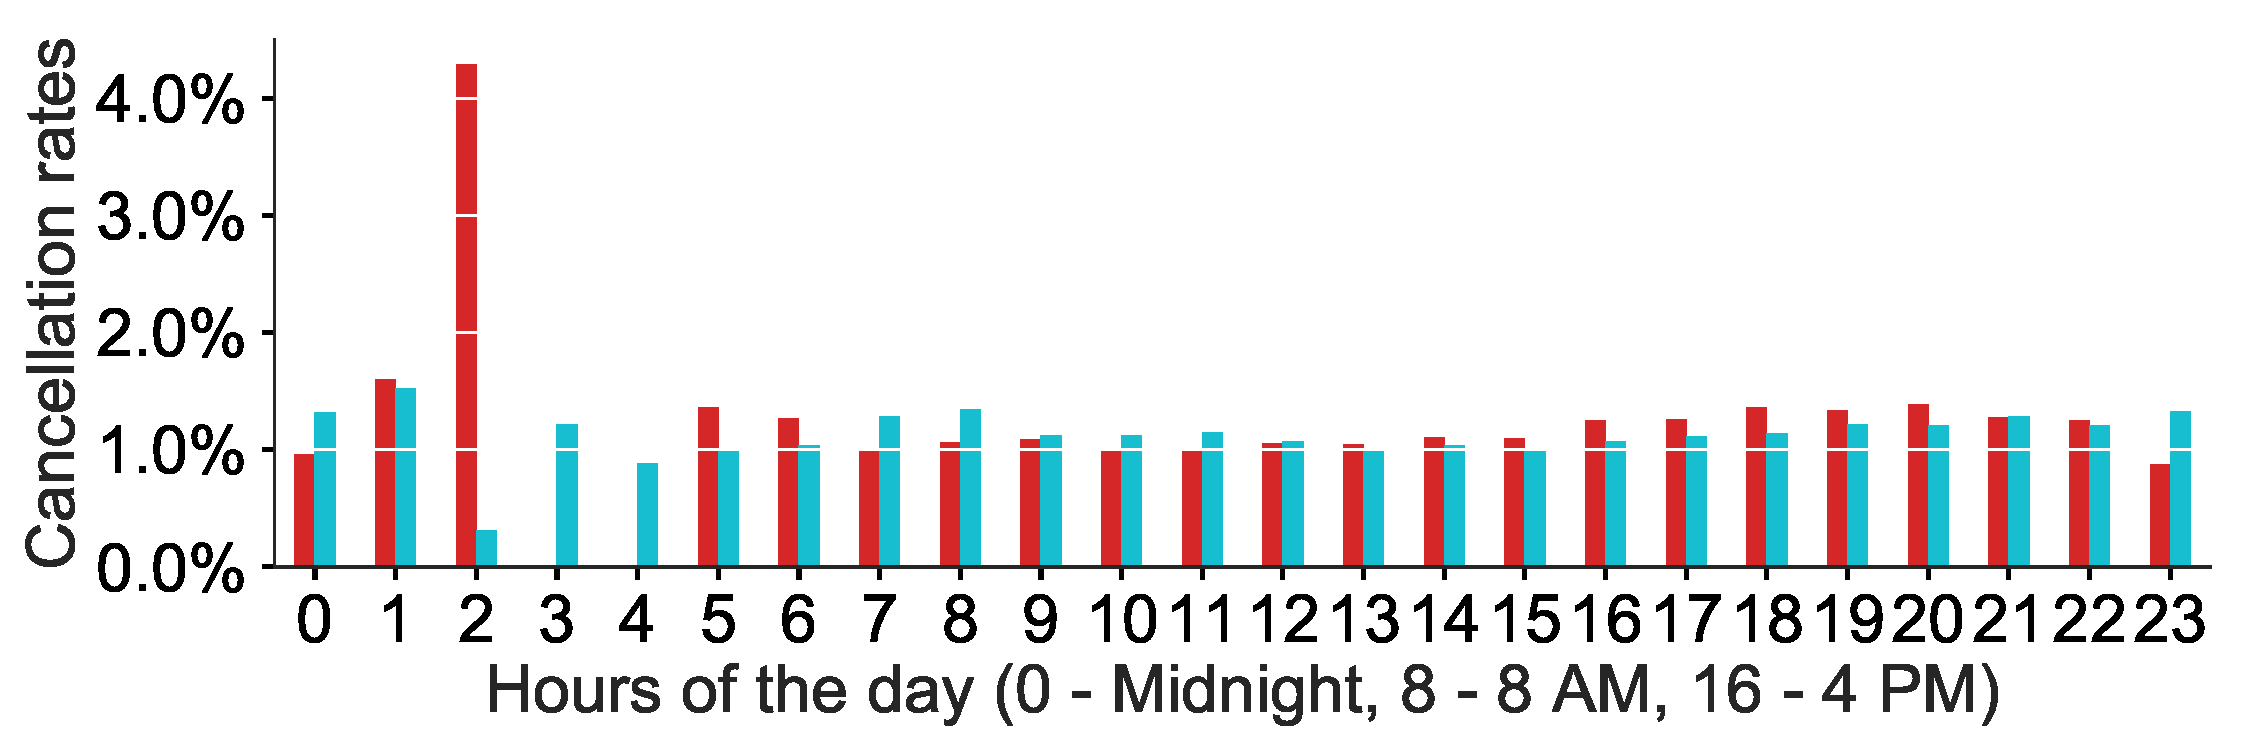
\includegraphics[width=6in]{hourly_canrate.pdf}
\end{center}
\caption{\label{fig:hourlycanrate}
Hourly cancellation rates throughout the day. Note the colors correspond to the same legend as in Fig.\ref{fig:monthlycanrate}.}
\end{figure}
For all scheduled departure hours, except between 2 - 3 AM, the cancellation rates are below $2\%$. We do not see any big spike in the case of scheduled arrival hours. Out of 210 flights scheduled to depart between 2-3 AM , 9 were cancelled, leading to spike at 2-3 AM red bar in the figure. This completes our brief discussion on calendar variables.
%%%%%%%%%%%%%%%%%%%%%%%%%
\subsection{Airports}
\label{subsec:airports}
%%%%%%%%%%%%%%%%%%%%%%%%%
We calculate the cancellation rates for flights departing from and arriving at all top 20 airports and display the results in Fig. \ref{fig:airportcanrate}. 
\begin{figure}[h!]
\begin{center}
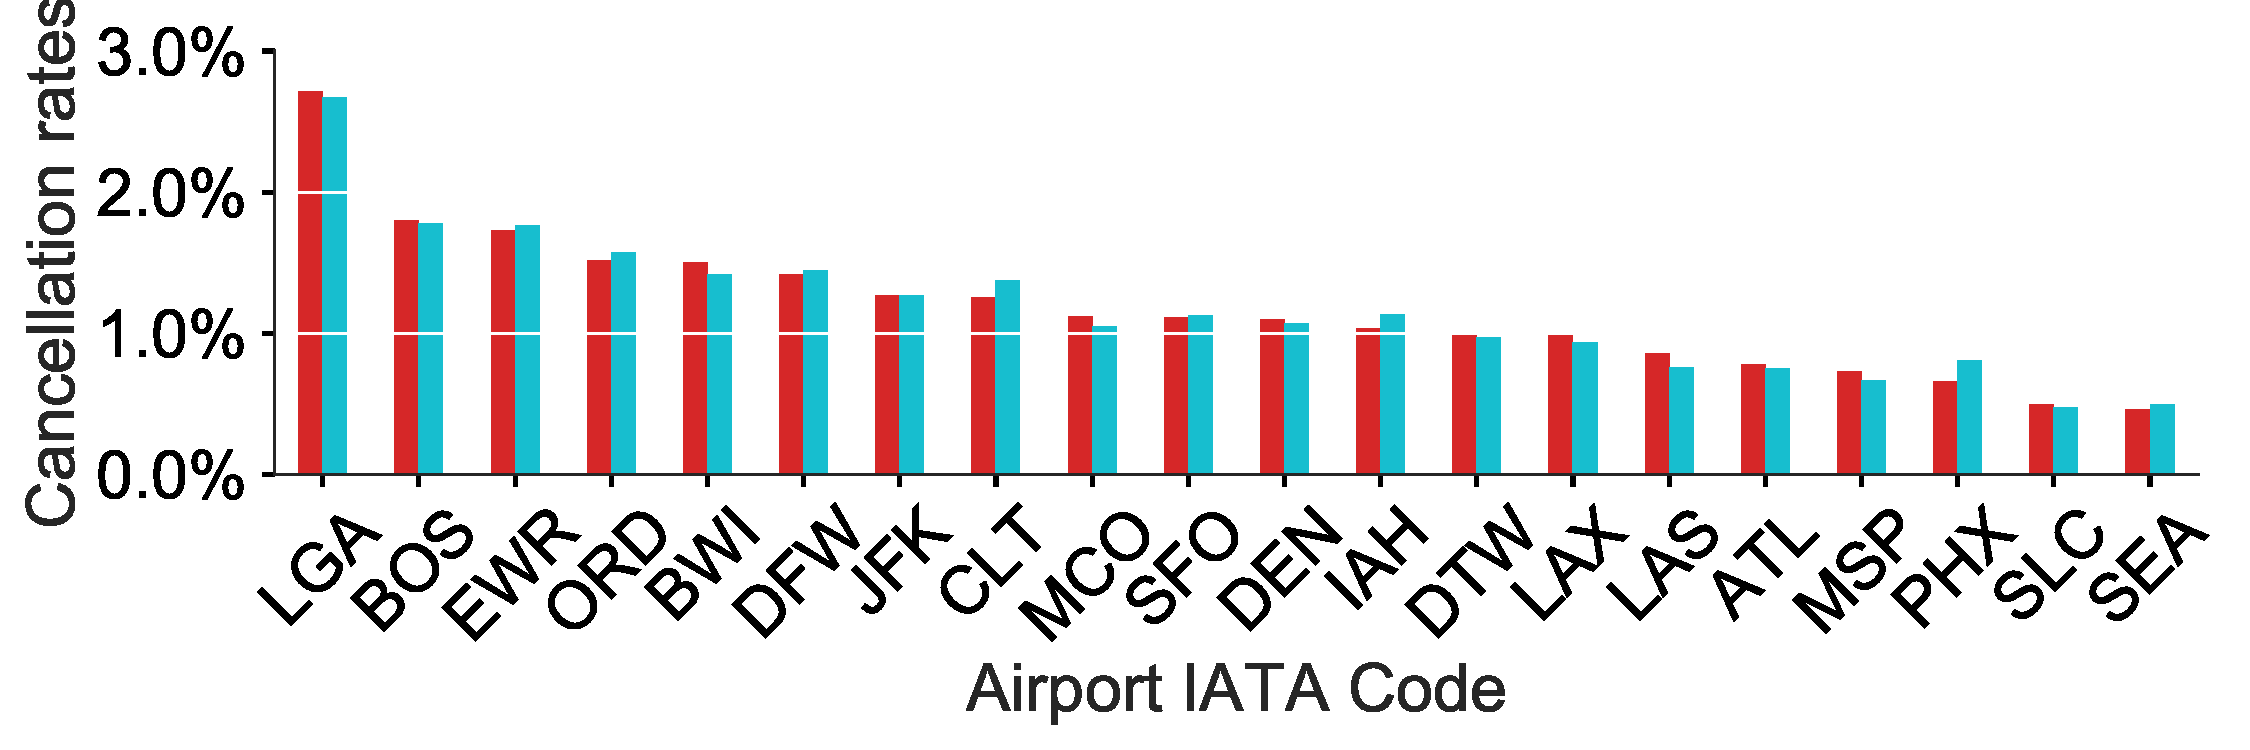
\includegraphics[width=6in]{airport_canrate.pdf}
\end{center}
\caption{\label{fig:airportcanrate}
Cancellation rates dependency on the airport. Note the colors correspond to the same legend as in Fig.\ref{fig:monthlycanrate}.}
\end{figure}
The IATA code can be found in \href{http://www.iata.org/publications/Pages/code-search.aspx}{this link}.
The flights departing from LaGuardia Airport (LGA) have the highest cancellation rate whereas the flights departing from Seattle - Tacoma International Airport (SEA) have lowest rate. The top 2 and the bottom 2 airports remain the same whether we are looking at origin or destination airport. 
%%%%%%%%%%%%%%%%%%%%%%%%%
\subsection{Airlines}
\label{subsec:airlines}
%%%%%%%%%%%%%%%%%%%%%%%%%
For airlines, it does not make sense to distinguish between the origin and destination. Figure \ref{fig:airlinecanrate} shows the cancellation rates for 13 airlines.  
\begin{figure}[h!]
\begin{center}
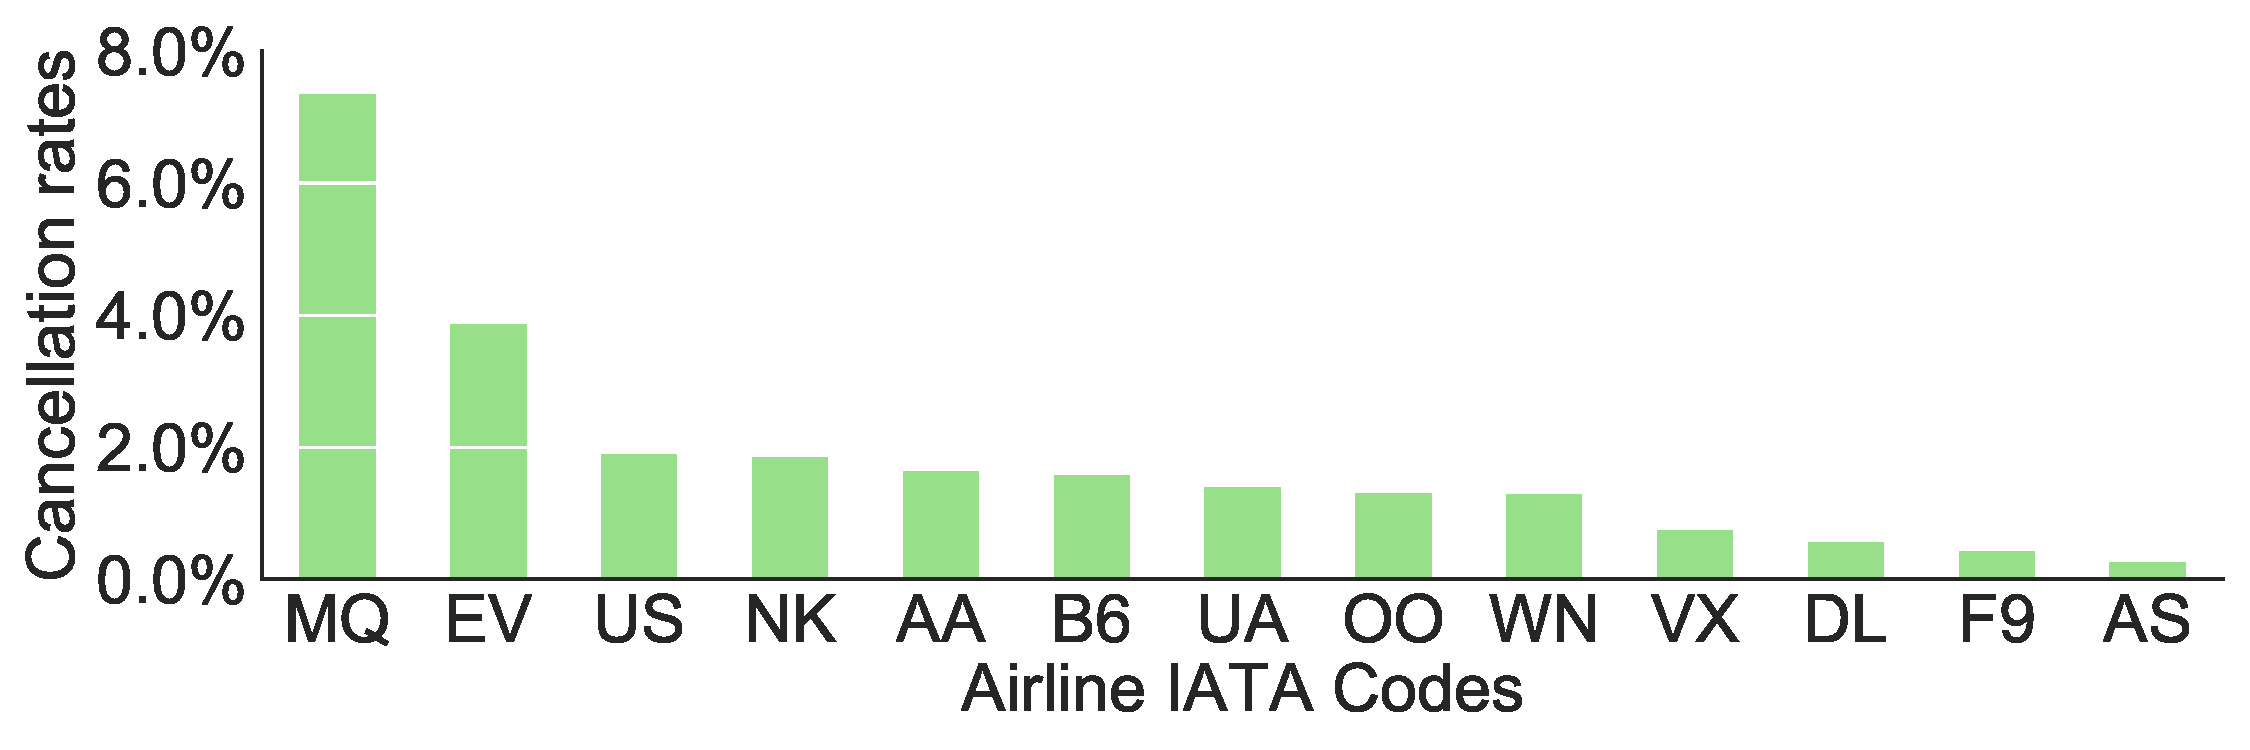
\includegraphics[width=6in]{airline_canrate.pdf}
\end{center}
\caption{\label{fig:airlinecanrate}
Cancellation rates dependency on the airline.}
\end{figure}
The airline IATA code can be found in \href{http://www.iata.org/publications/Pages/code-search.aspx}{this link}. The highest cancellation rate is seen for the Envoy Air (MQ), and lowest is seen for the Alaska Airlines (AS). Two airlines with highest cancellation rates (MQ and EV) are not mainline airlines but rather regional ones. OO (SkyWest Airlines) is also regional airline but has relatively lower cancellation rates.
%%%%%%%%%%%%%%%%%%%%%%%%%
\subsection{Flight Distance}
\label{subsec:flightdistance}
%%%%%%%%%%%%%%%%%%%%%%%%%
Flight distance is recorded in miles and is a continuous variable. For every numerical value of this variable, we calculate the cancellation rate, which is shown in Fig. \ref{fig:distancecanrate}.   
\begin{figure}[h!]
\begin{center}
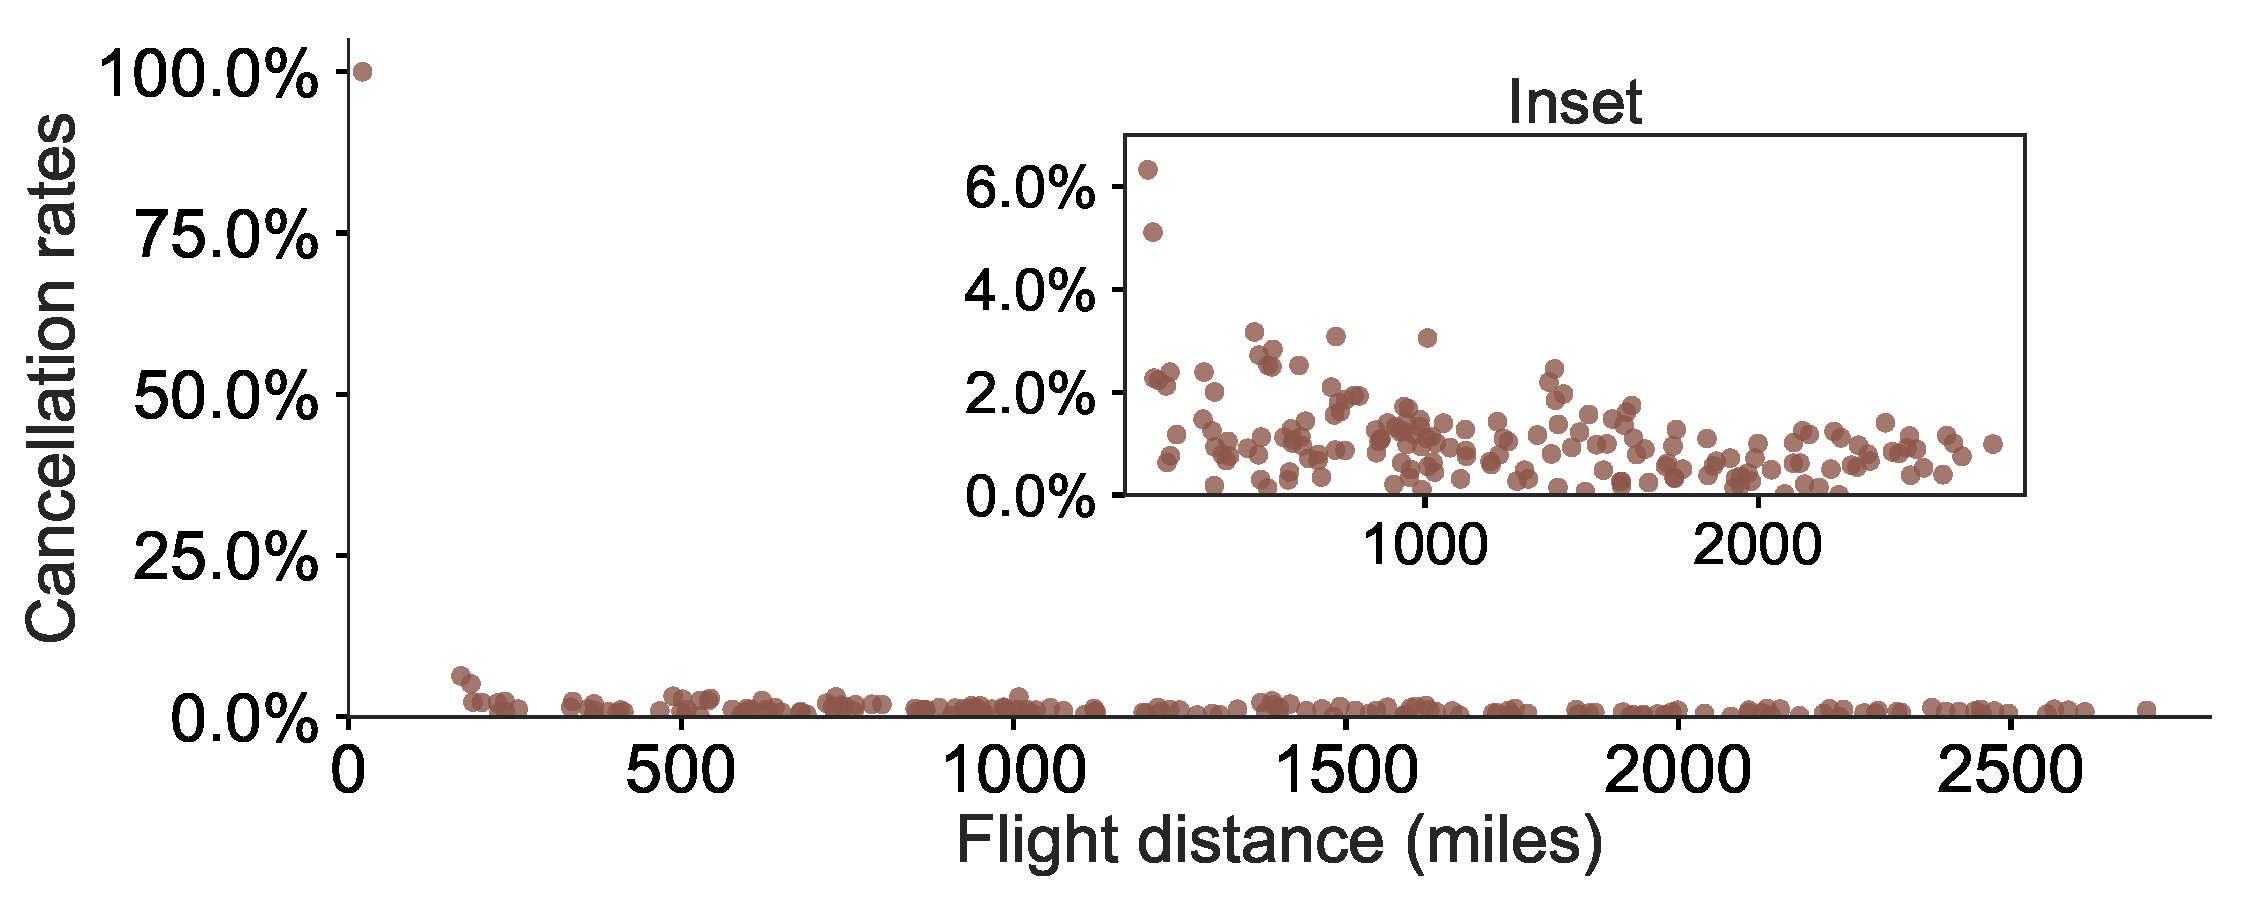
\includegraphics[width=6in]{distance_canrate.pdf}
\end{center}
\caption{\label{fig:distancecanrate}
Cancellation rates as a function of flight distance.}
\end{figure}
There is a data point for Distance = 21 miles for which the cancellation rate was 100$\%$. In order to see the clear trend for all other data points, we omitted the 21 miles point and replotted the data in the inset figure. We can see that the cancellation rates are higher for shorter distance flights and lower for longer distance flights. We performed a hypothesis test to test the null that there is no relationship between the distance and the cancellation rate. Using Spearman's $\rho$, we found a weak correlation of -0.39 which was statistically significant. 
%%%%%%%%%%%%%%%%%%%%%%%%%
\subsection{Weather Factors}
\label{subsec:weatherfactors}
%%%%%%%%%%%%%%%%%%%%%%%%%
There are many weather factors such as temperature, dew point, pressure, wind speed, wind direction, humidity etc.. but we will focus on only some factors here to keep the discussion short. A detailed data exploration can be found in \href{https://github.com/aajains/springboard-datascience-intensive/blob/master/capstone_project/EDA/ExploratoryDataAnalysis.ipynb}{this IPython notebook}. 


Fig. \ref{fig:tempcanrate} displays the cancellation rate asa function of temperature at both origin and destination (at the time of departure and arrival, respectively). There appears to be two broad temperature regimes here in terms of cancellation rates. The cancellation rates are four times higher when the temperatures are below 40 $^\circ$F as compared to the situations when temperatures above 40 $^\circ$F. which can be clearly seen in the inset figure. 
\begin{figure}[h!]
\begin{center}
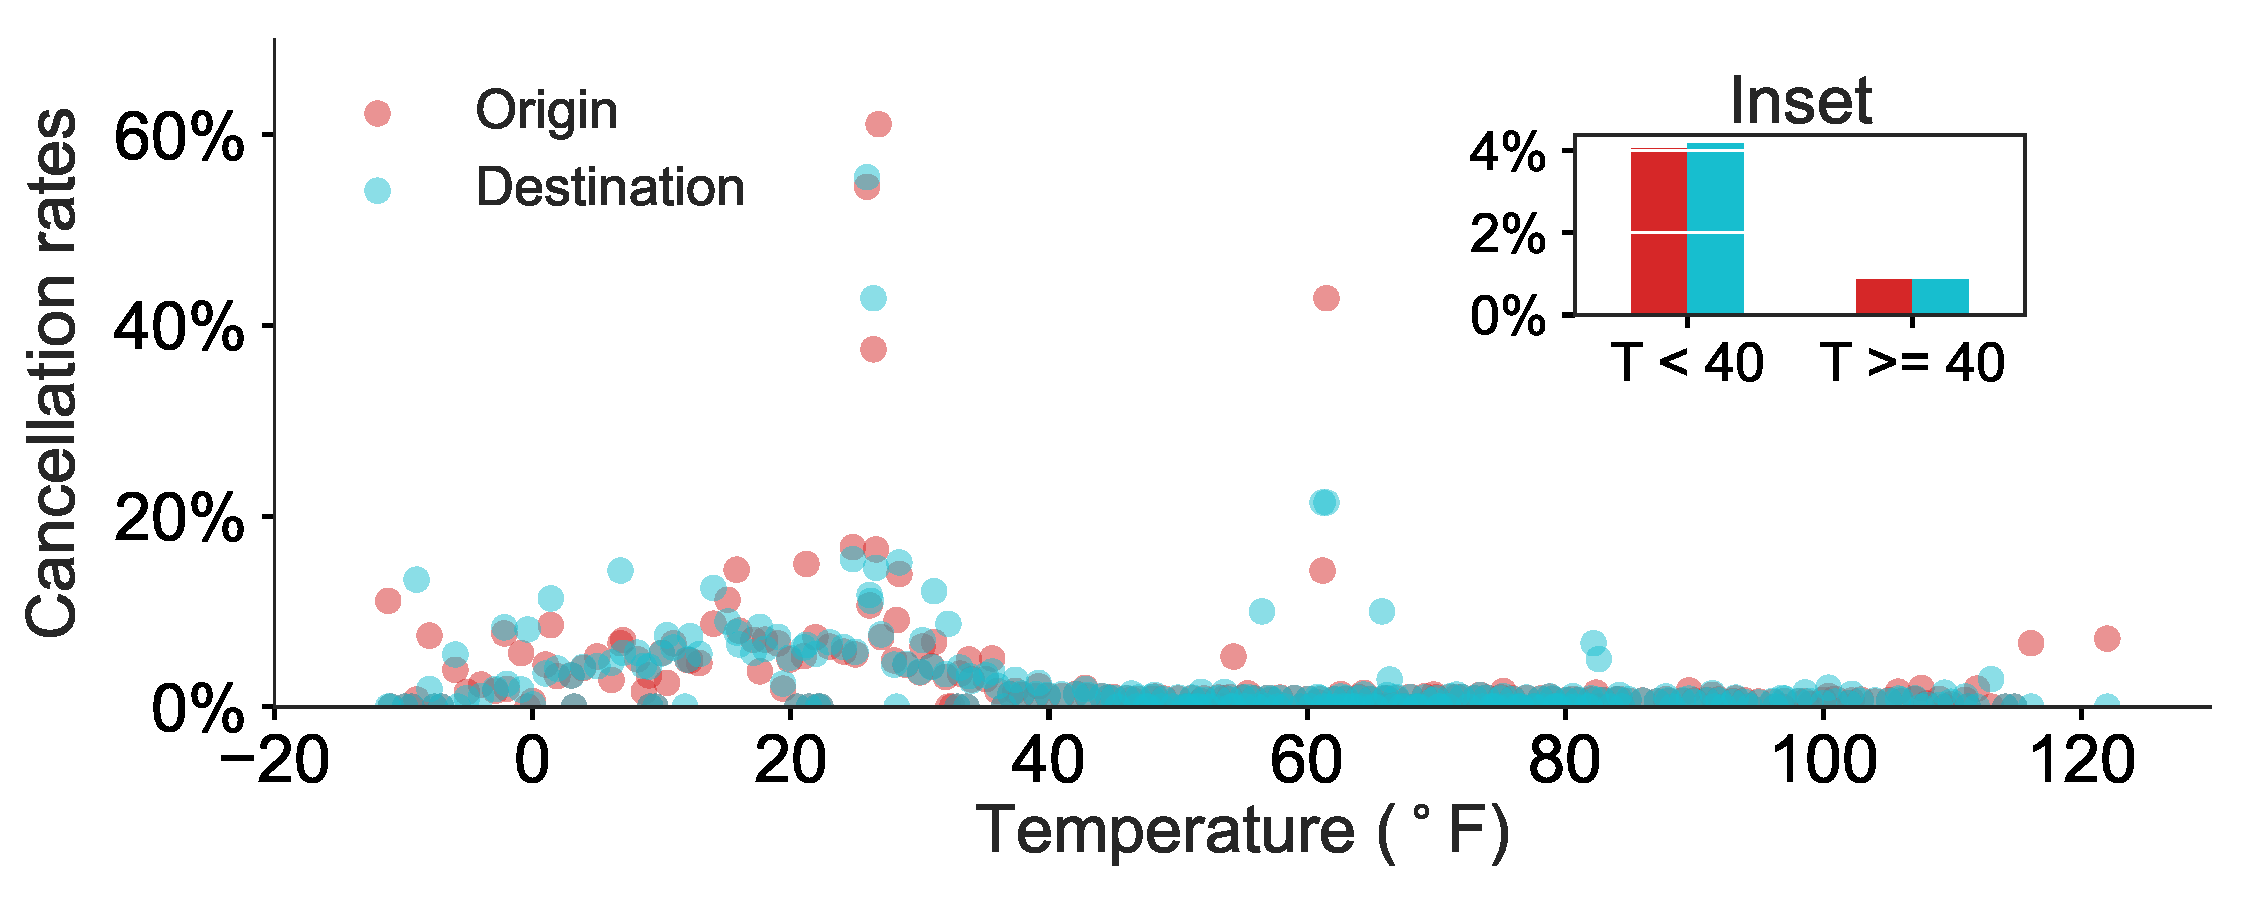
\includegraphics[width=6in]{temperature_canrate.pdf}
\end{center}
\caption{\label{fig:tempcanrate}
Cancellation rate as a function of temperature. In the inset bar chart, y-axis is for the cancellation rate and $T$ represents temperature.}
\end{figure}
Humidity and wind speed have similar effects on cancellation rates as shown in Fig. \ref{fig:humwindcanrate} for both origin and destination locations. For very dry weather conditions (less than 10$\%$), there is a decreasing trend for cancellation rate. The rate then monotonically increase for humidity more than 20$\%$. For the monotonic part, we found statistically significant values of Spearman's correlation $\rho$ to be around 0.79 for origin and 0.82 for destination. 
\begin{figure}[h!]
\begin{center}
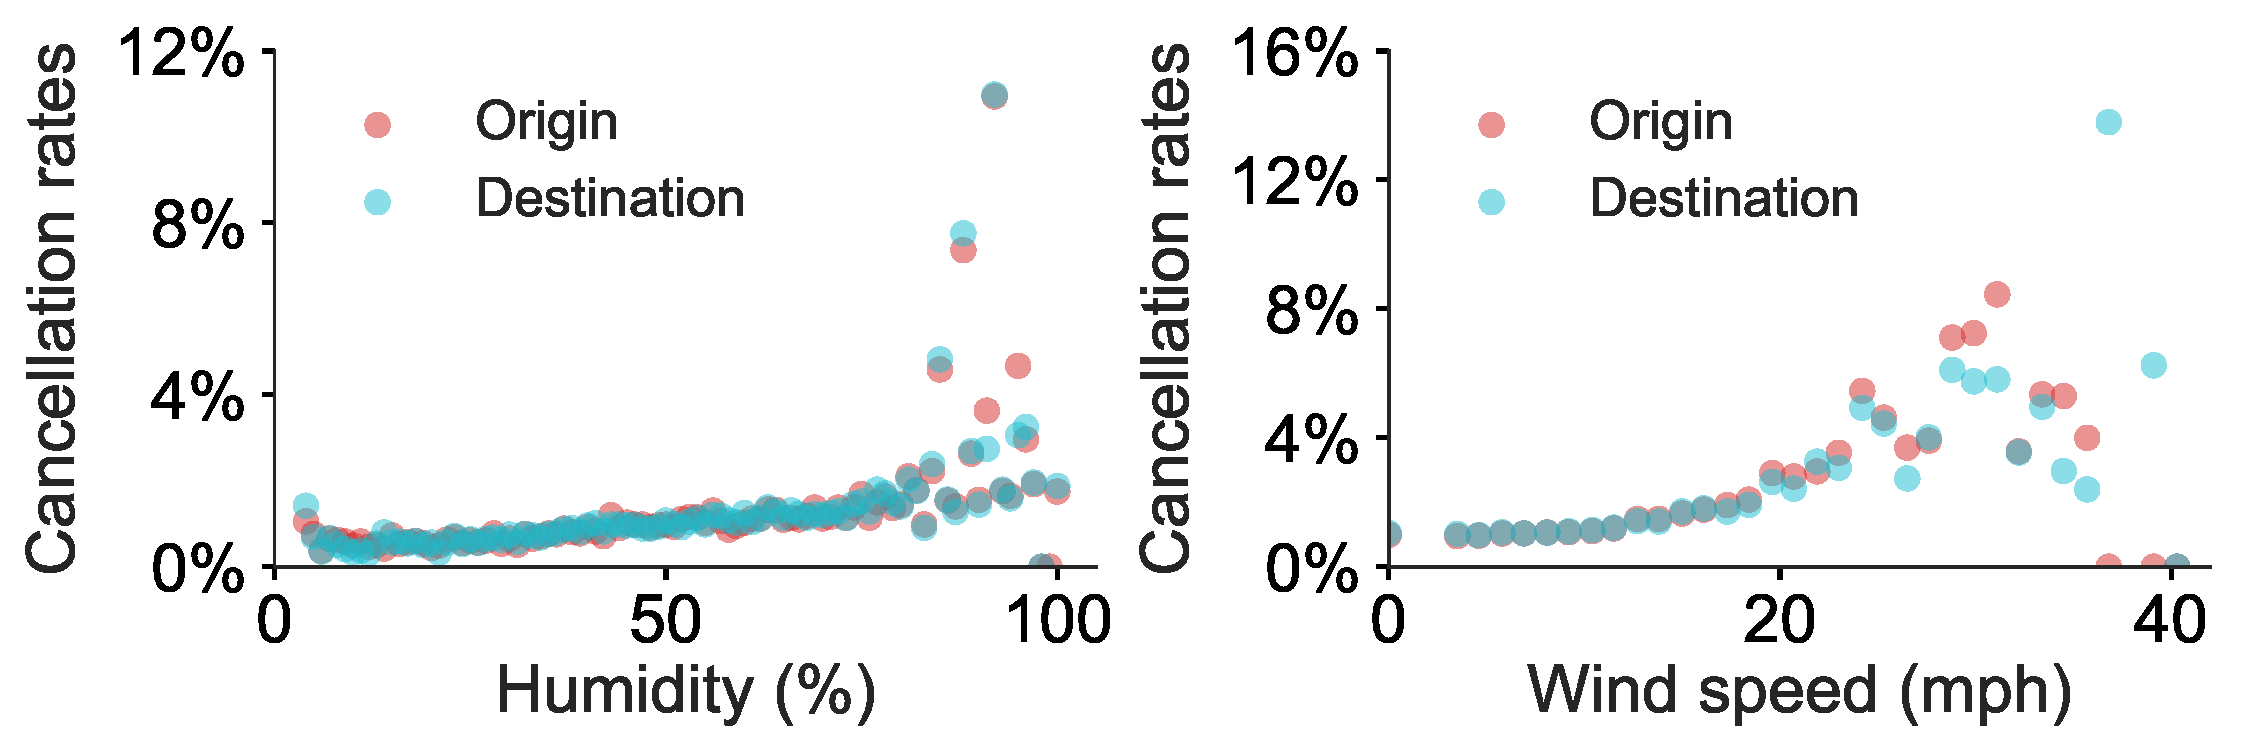
\includegraphics[width=6in]{humidity_windspeed_canrate.pdf}
\end{center}
\caption{\label{fig:humwindcanrate}
Cancellation rate as a function of $\%$ humidity and wind speed (mph).}
\end{figure}
Also, we see a monotonically increasing trend for cancellation rates as a function of wind speed until around 25 mph. For wind speed greater than that, the cancellation rates start to decrease. The maximum point for cancellation rates are different for origin and destination airports. Overall, the trends are pretty much like parabolic curves for wind speed.


We now look at the wind direction in FIg. \ref{fig:winddircanrate}. It turns out that from 90 to 270 degrees, i.e. from East to South to West, the cancellation rates are around 1$\%$. When the wind direction goes from West to close to North, the cancellation rates increased. The rates fluctuate a lot when the wind direction is close to North. From North to Wast wind direction, the cancellation rate start to decrease.
\begin{figure}[h!]
\begin{center}
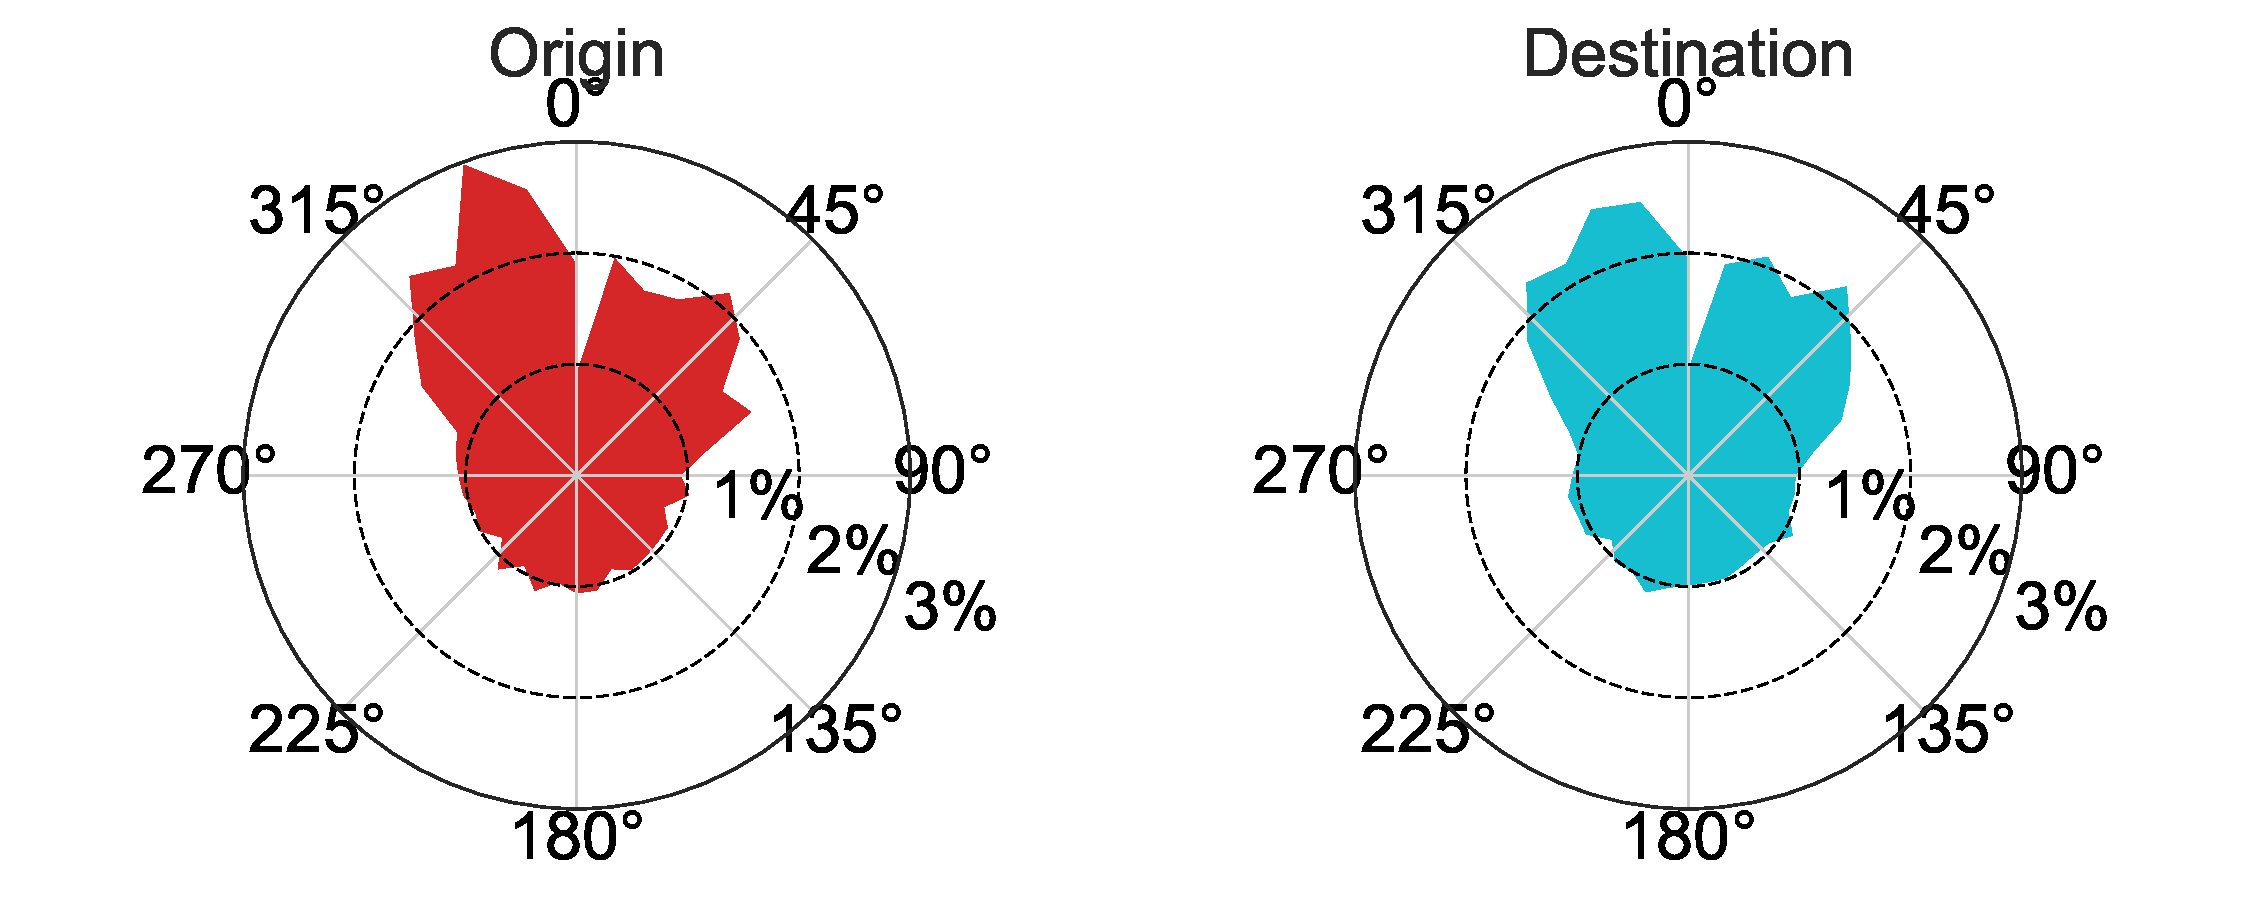
\includegraphics[width=6in]{winddir_canrate.pdf}
\end{center}
\caption{\label{fig:winddircanrate}
Cancellation rate as a function of wind direction. 0$^\circ$ corresponds to North, 90$^\circ$$\%$ to East, 180$^\circ$ to South and 270$^\circ$ to West.}
\end{figure}
Finally, we look at various weather conditions and find out the cancellation rates under all conditions, as displayed in Fig. \ref{fig:conditionscanrate}.
\begin{figure}[h!]
\begin{center}
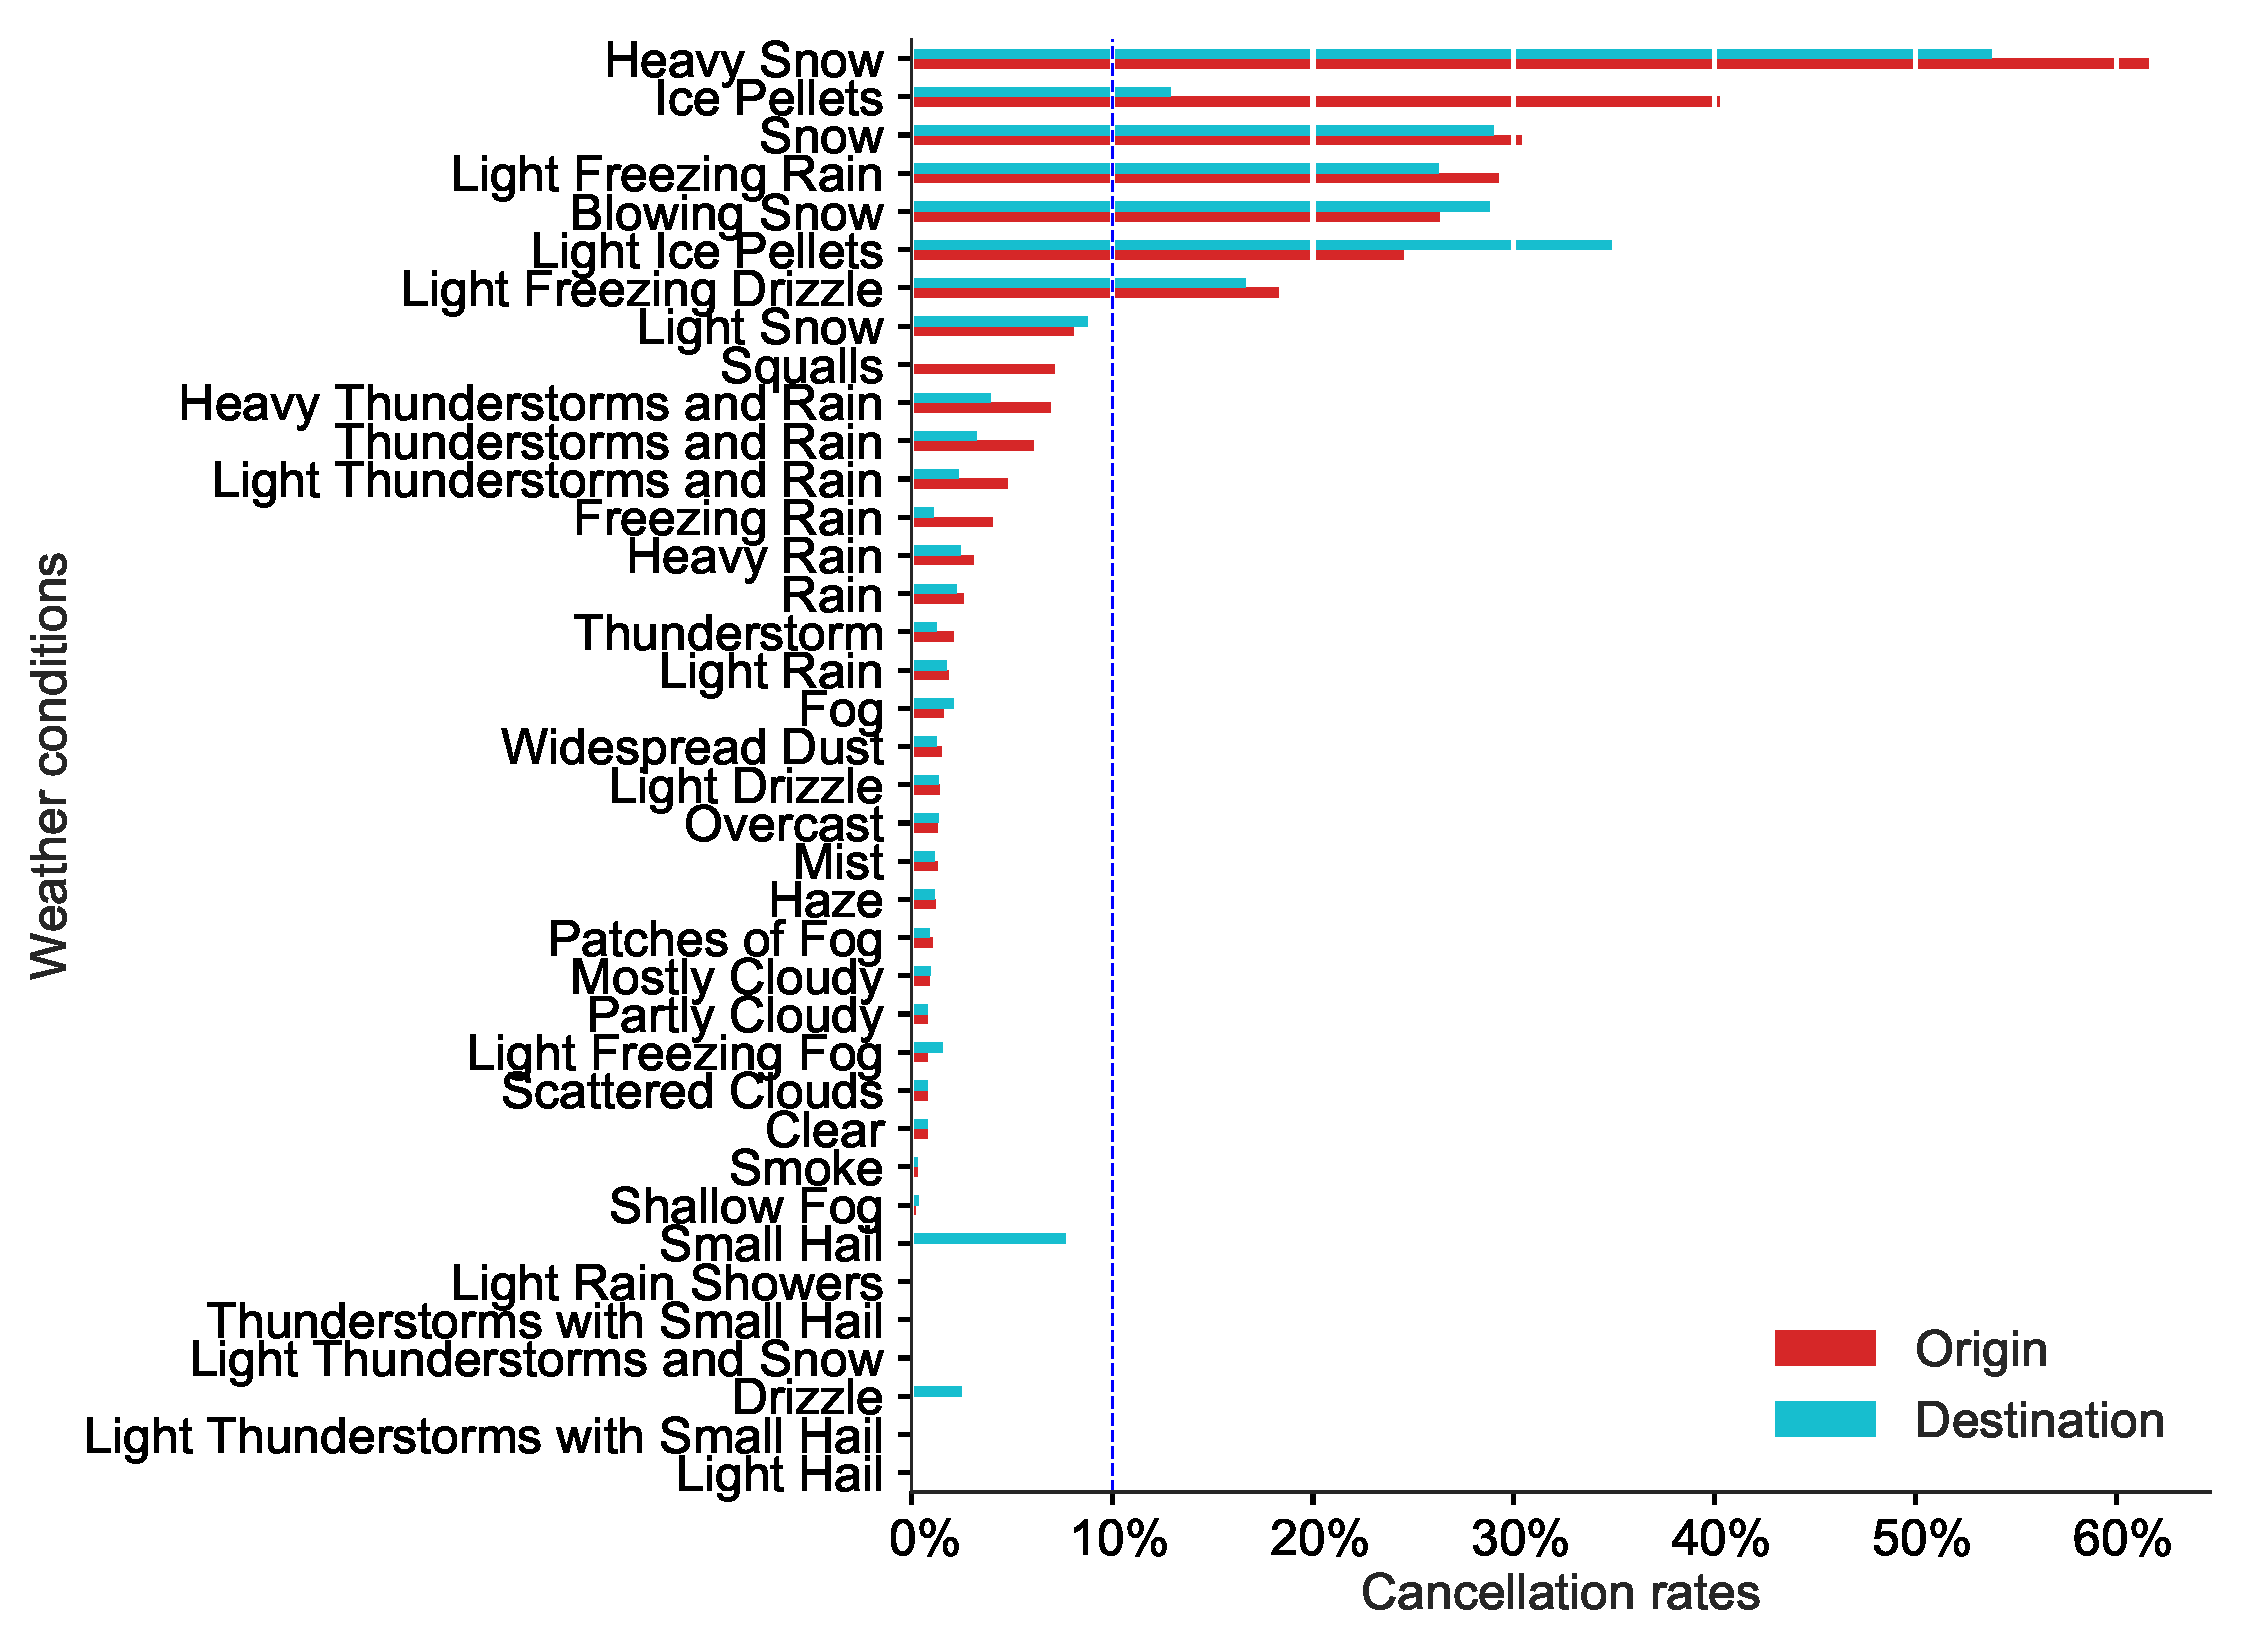
\includegraphics[width=6in]{conditions_canrate.pdf}
\end{center}
\caption{\label{fig:conditionscanrate}
Cancellation rates under different weather conditions at origin and destination airports. The dashed vertical blue line indicates 10$\%$ cancellation rate line.}
\end{figure}
Cancellation rates are pretty high when there are snow related activities at both origin and destination airports. Rain with some thunderstorms also has high cancellation rates. There are similar top weather factors for both locations for cancellation rates greater than 10$\%$ (indicated by blue dashed line), with an exception such as ``Squalls" which has very low cancellation rate at destination and high rates at the origin airports. However, this observation is not significant as there are only 28 records for Squalls at origin. Similarly, the cancellation rates are almost 0 when there are any type of hail conditions. Again, the number of records containing this condition is 69 at origin, so this observation is also not significant.
%%%%%%%%%%%%%%%%%%%%%%%%%
\subsection{Historical Performances}
\label{subsec:historical}
%%%%%%%%%%%%%%%%%%%%%%%%%
For historical performances of a given flight, we have the number of cancellations, number of diversions, departure delays, arrival delays and taxi times for last ``ndays", where we have three values of ndays = 10, 20 and 30. Figure \ref{fig:candivcanrate} shows the influence of the number of cancellations and diversions in the last ndays on the cancellation rate of the flight in question. Each data point in this figure is the result of some calculations. For example, to calculate the cancellation rate for a given number of cancellations ($N_c$), we pick all the flights for which the number of cancellations were $N_c$ in the last ndays. We then count the number of such flights, and also the number of cancelled flights. The ratio then gives us the cancellation rate for $N_c$. We can perform the similar steps for all other historical performance variables but let us first discuss Fig. \ref{fig:candivcanrate}.
\begin{figure}[h!]
\begin{center}
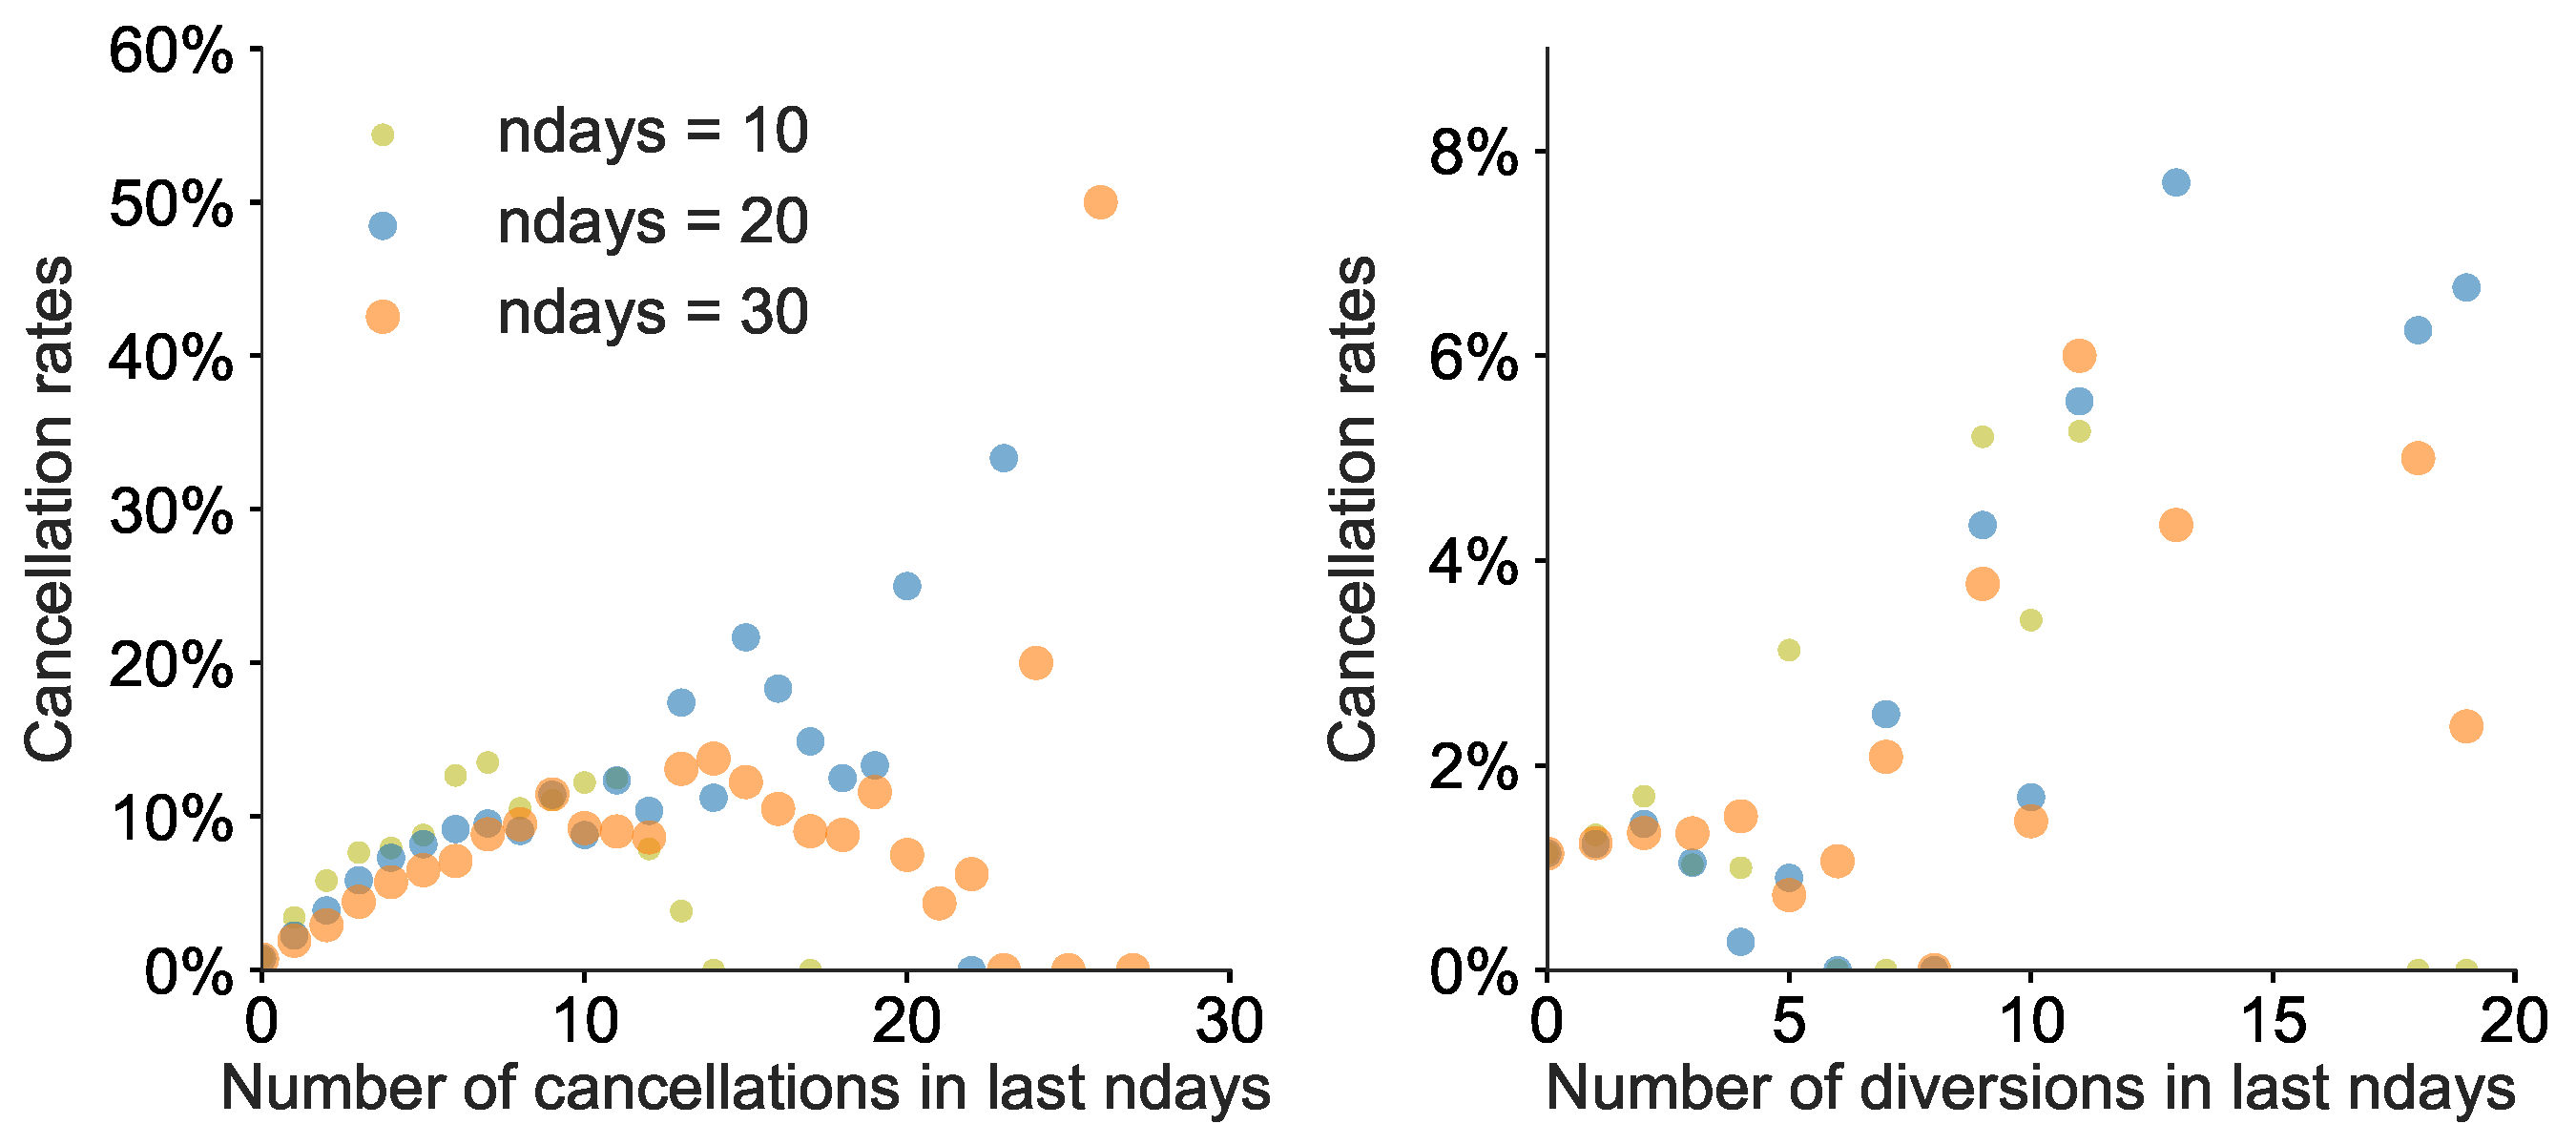
\includegraphics[width=6in]{candiv_canrate.pdf}
\end{center}
\caption{\label{fig:candivcanrate}
Cancellation rates as a function of the number of cancellations and the number of diversions in the last ndays.}
\end{figure}
For the left panel figure, we observe a parabolic pattern with maximum in cancellation rates occurring at different values of the number of cancellations for different values of ndays. There also appears to be some outliers in all three cases, usually at higher values of the number of cancellations in last ndays.
For the right panel figure, generally, the cancellation rates for a flight is higher when the number of diversions of that flight in the last ndays are higher.


Sometimes, we come across a flight for which we do not find any history in the last ndays. We call such flights as temporary flights. The term ``temporary" could be different for different ndays. For example, a flight can be temporary if looked at 10 days history but ``routine" if looked at 30 days history. Figure \ref{fig:historyindicatorcanrate} (a) compares the cancellation rates for temporary (Yes) and routine (No) flights  for all three ndays. Usually, the cancellation rates are higher for temporary flights.  
\begin{figure}[h!]
\begin{center}
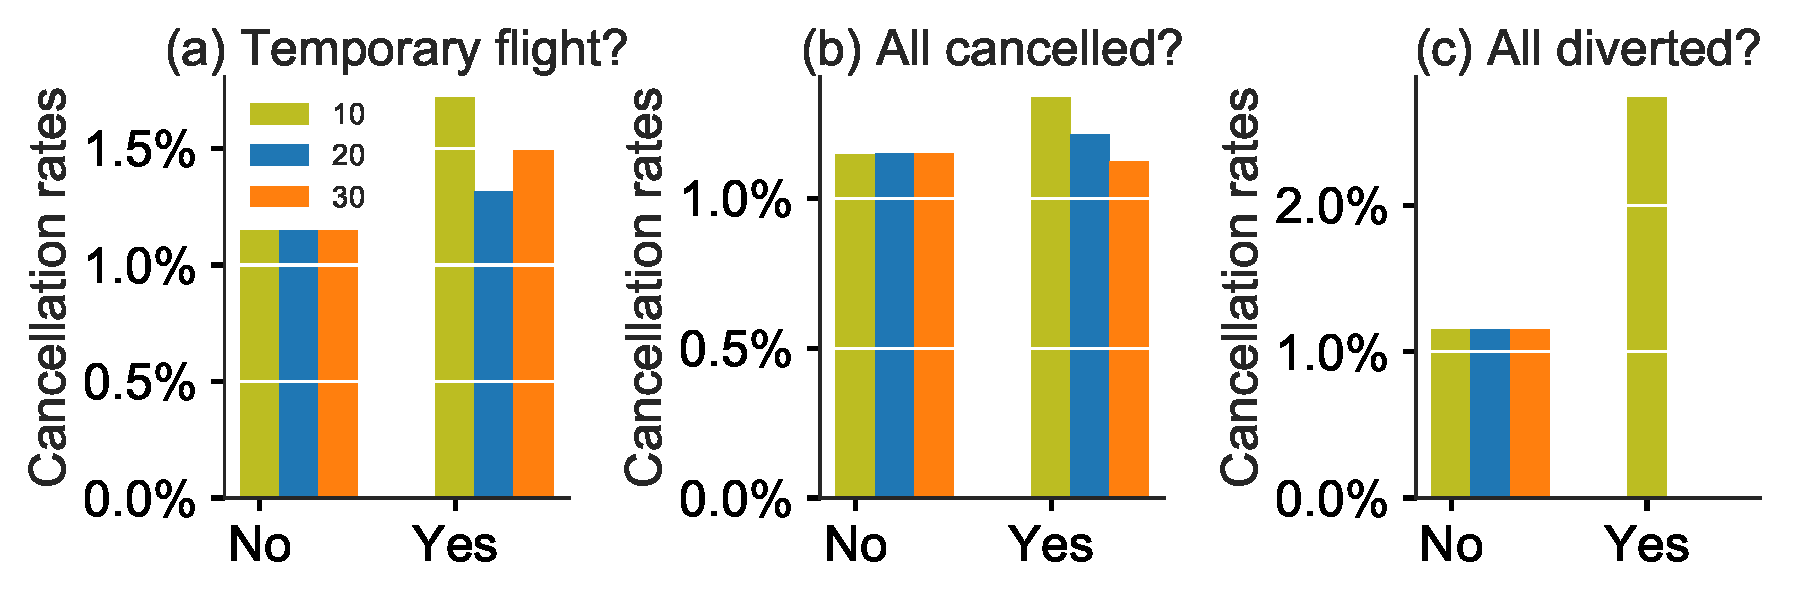
\includegraphics[width=6in]{history_indicator_canrate.pdf}
\end{center}
\caption{\label{fig:historyindicatorcanrate}
Cancellation rate comparisons for three different history indicators, and for all three ndays. The legend 10, 20 and 30 indicates different ndays.}
\end{figure}
There are also some flights for which the history tells that all the flights in last ndays got cancelled. The cancellation rates are slightly higher when all flights got cancelled in the last ndays, as seen in Fig. \ref{fig:historyindicatorcanrate} (b). Similarly, there are flights for which there were 100$\%$ diverted flights in the last ndays. We found such cases only for ndays=10 and the cancellation rates are about 3 times higher as compared to the flights for which the history had no 100$\%$ diversions, as shown in Fig. \ref{fig:historyindicatorcanrate} (c).


Now, we look at the influence of departure delays statistics on cancellation rates. Figure \ref{fig:depdelaymediancanrate} presents the cancellation rates for given median values of the departure delays in the last ndays. 
\begin{figure}[h!]
\begin{center}
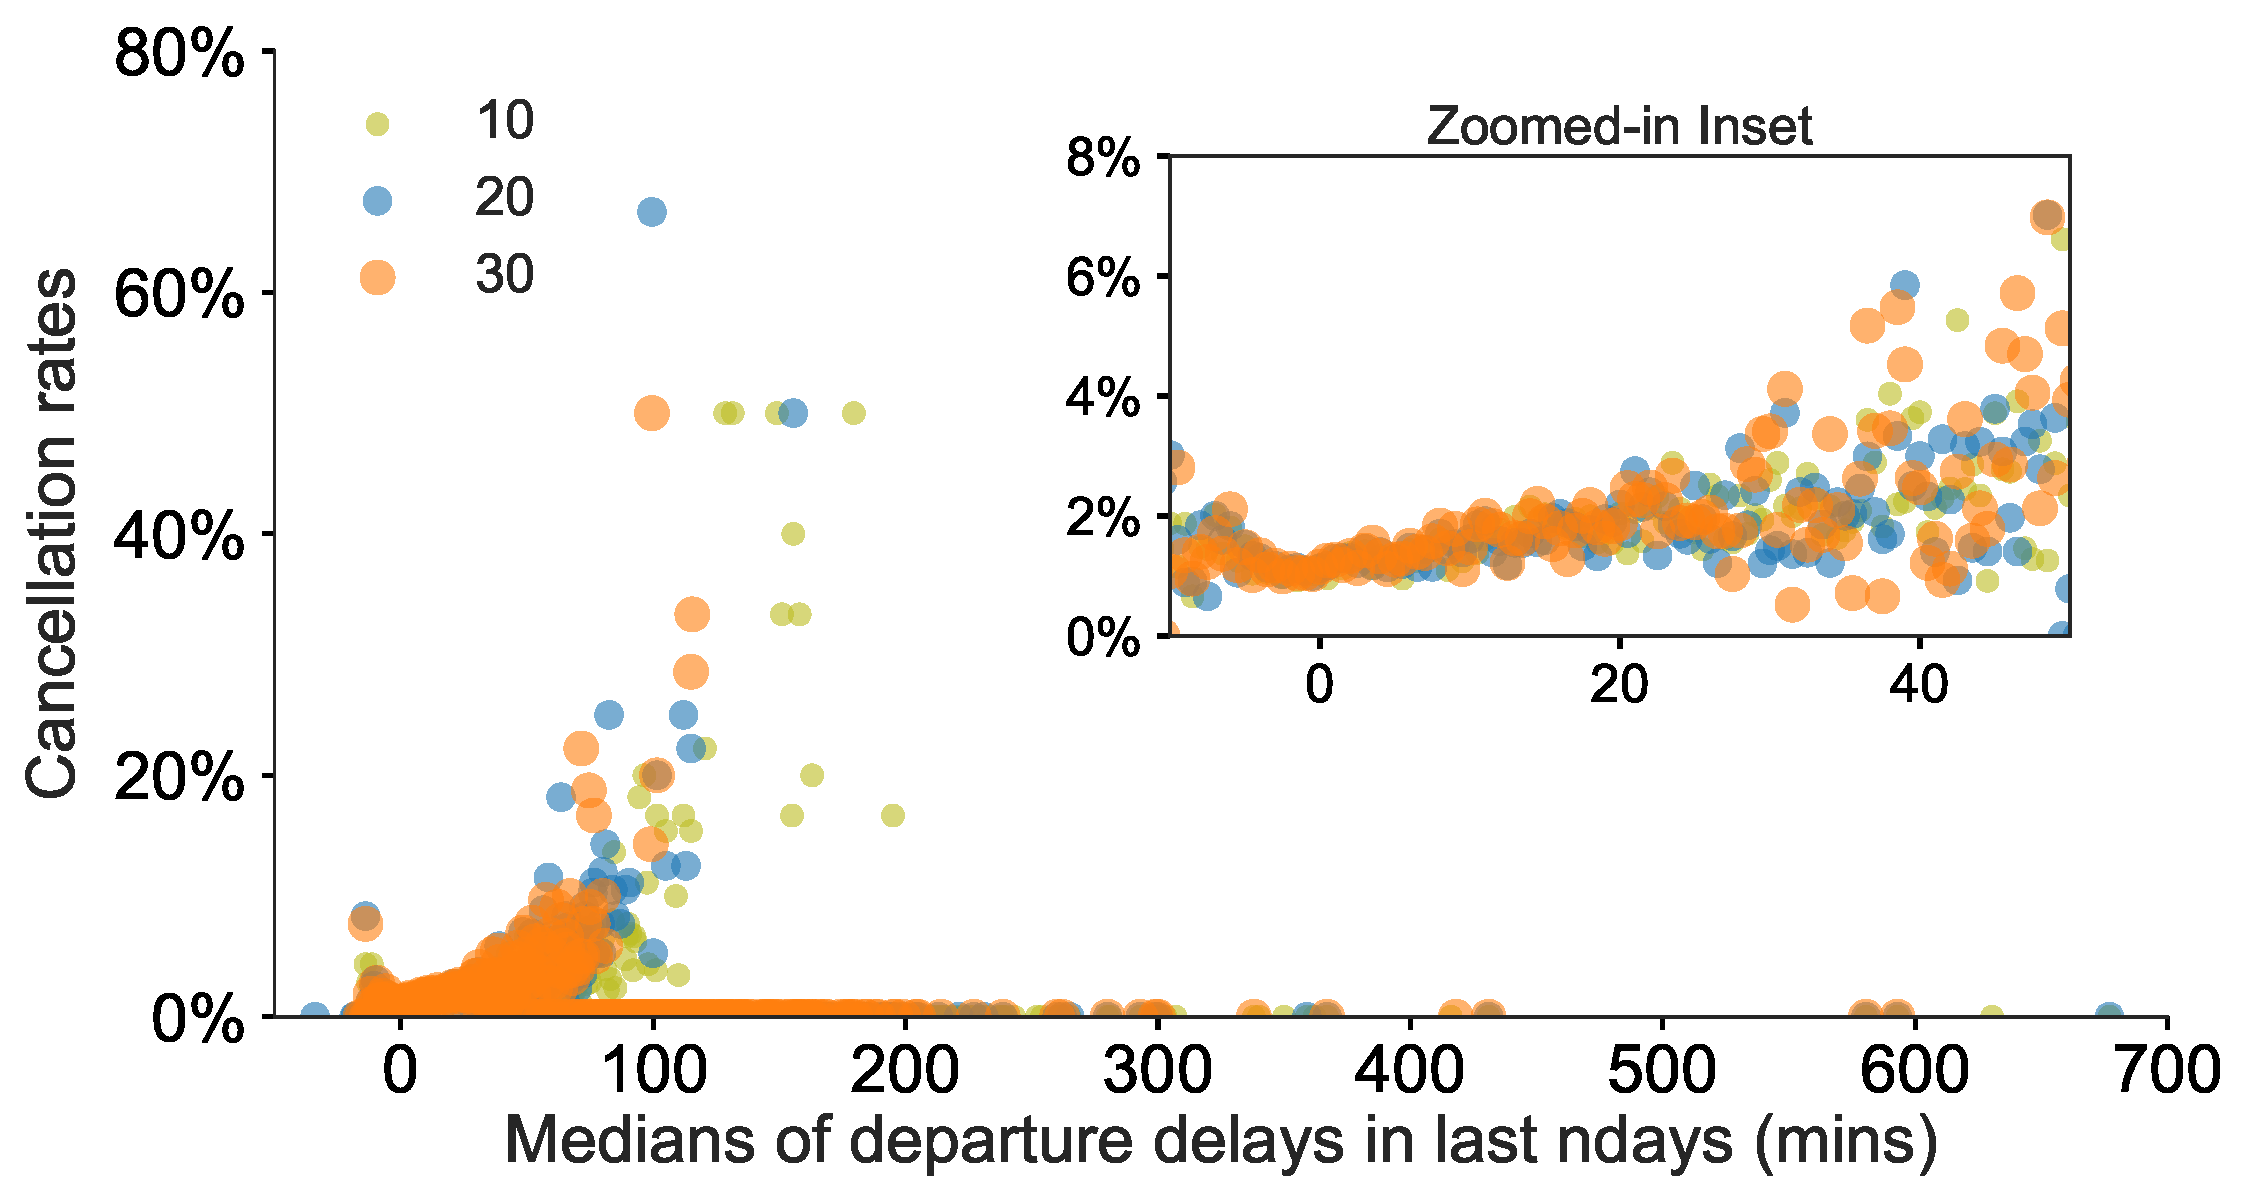
\includegraphics[width=6in]{depdelaymedian_canrate.pdf}
\end{center}
\caption{\label{fig:depdelaymediancanrate}
Cancellation rates as a function of the medians of departure delays in the last ndays. The legend 10, 20 and 30 indicates different ndays. The inset figure has the same x and y labels as the main figure.}
\end{figure}

Cancellation rates are 0 (except a couple of instances) when the medians of departure delays in last ndays days were greater than 200 minutes. For less than 200 mins, and more specifically between 0 and 70 mins, there is a somewhat increasing cancellation rate as a function of median values, as displayed in the inset figure. Statistically significant correlations (Spearman's $\rho$ = 0.77, 0.69, 0.55, for ndays = 10, 20, 30, respectively) are found for all three ndays data in 0-70 mins range.  


In a similar fashion, we can also look at the effect of medians of arrival delays in Fig. \ref{fig:arrdelaymediancanrate}.
\begin{figure}[h!]
\begin{center}
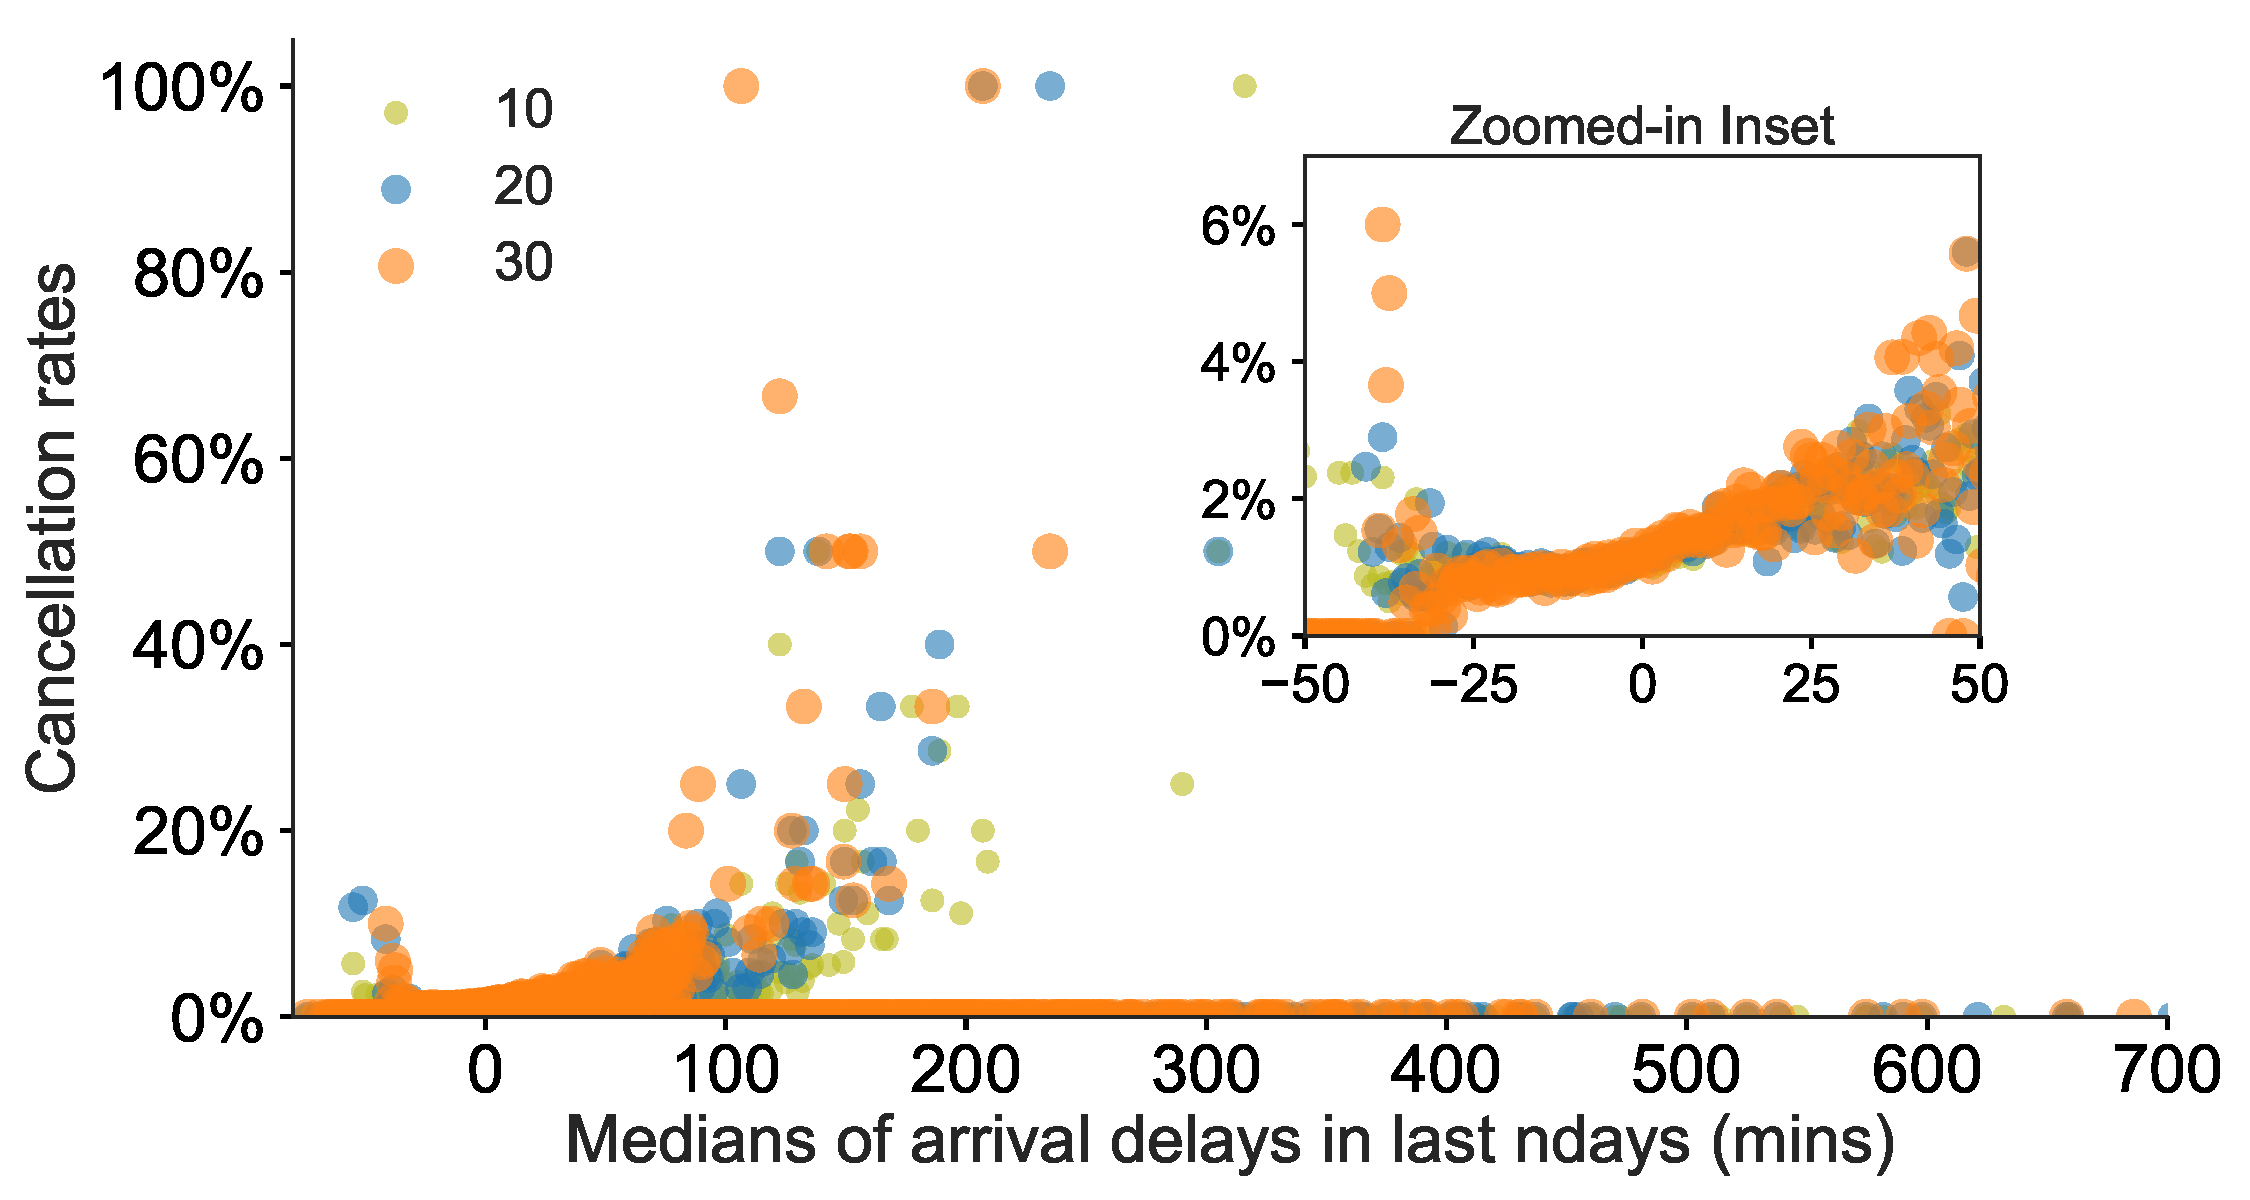
\includegraphics[width=6in]{arrdelaymedian_canrate.pdf}
\end{center}
\caption{\label{fig:arrdelaymediancanrate}
Cancellation rates as a function of the medians of arrival delays in the last ndays. The legend 10, 20 and 30 indicates different ndays. The inset figure has the same x and y labels as the main figure.}
\end{figure}
This scatter plot looks very similar to the one that we got for medians of departure delays. For more than about 200 mins arrival delays, the cancellation rates are 0 for any ndays history. However, when we zoom-in the plot between -50 to 50 mins, we observe a non-monotonic behavior.   
%%%%%%%%%%%%%%%%%%%%%%%%%
\section{Limitations}
\label{sec:limit}
%%%%%%%%%%%%%%%%%%%%%%%%%
There are some limitations in the data which would reduce the robustness of the machine learning model that we will develop.
\begin{enumerate}
\itemsep0em
\item We have considered only 20 airports in this project due to weather data provider's API restrictions. Though 20 airports broadly cover the whole US, a lot of information will not be learned by the model due to the absence of all airports in the dataset. 
\item The prediction of the model will depend on how good the prediction of the weather is, say after 3 days. In other words. if we want to predict the likelihood of the flight cancellation for a flight which is scheduled after 3 days, we would need to know the weather after 3 days (which we do not know ``accurately" today). This means that the model will predict better if the weather prediction is better or if we are trying to predict the flights not far ago than the scheduled departure.
\item Apart from knowing whether a flight was cancelled, we also have information about the cancellation codes such as A, B, C, D. Most probably these codes correspond to different reasons or factors for cancellation. However, other than just knowing these codes, we do not know the exact meanings of these codes. If the exact meanings were known, we would have built a multi-class classification model. Lack of this information restricts us to develop a binary classifier only.  
\item We found that SunCountry Airline (IATA code: SY) data is missing in the original flight dataset which we acquired from the \href{https://www.transtats.bts.gov/DL_SelectFields.asp?Table_ID=236&DB_Short_Name=On-Time}{Bureau of Transportation Statistics}. We checked for the absence of only this airline from a personal travel experience. It is possible that some other data might also be missing in the original dataset. Therefore, we emphasize that the analysis carried out in this project is only based on the data source that we mentioned here. 
\end{enumerate}
%%%%%%%%%%%%%%%%%%%%%%%%%
\section{Other Data and Future Work}
\label{sec:otherdata}
%%%%%%%%%%%%%%%%%%%%%%%%%
Other than the original flight data, weather data and historical performance data, we can also acquire or feature engineer more datasets which might enhance the predictive power of the machine learning model. Knowing the airport name, we can extract informations such as number of runways, runway length (and width), airport type, airport infrastructure, airport capacity etc.., and create new features. Similarly, knowing the airlines names, we can extract airlines ratings, their stock market performance, their revenue and assets, reputations etc.., and create new fields. We can also get data from social networking sites and news media about the sentiment for each airlines and airports. The sentiment analysis can then be used to create more features. Datasets containing world events such as catastrophic natural destruction, terror attacks, political movement, sport tournaments, etc.. can also be acquired and used to merge with our original datasets. Each one of these ideas can be difficult if the data is not easily accessible. However, we believe that the predictive power of the model will be improved by incorporating these factors.  
%%%%%%%%%%%%%%%%%%%%%%%%%%%%%%%%%
\section{Conclusions}
%%%%%%%%%%%%%%%%%%%%%%%%%%%%%%%%%%%
We have explored the original flight dataset along with the merged weather datasets and engineered historical performance variables, to understand their influence on the flight cancellation rates. Top 20 airports (in terms of the number of flights operating) were considered in this work for the year 2015. The overall cancellation rate was about 1.28$\%$, which is not a large number but that is what makes the project more interesting. We explored 6 types of informations available in the datasets and found that most of them influence cancellation rates. Following is a quick summary of our findings:
\begin{enumerate}
\itemsep0em
\item \textbf{Calendar variables:} Most flights were cancelled in the winter months and least in the falls months. We also found that the cancellations are worst in the end and beginning of a week.
\item \textbf{Airports:} Usually the airports in the east coast had higher cancellation rates as compared to the rest of the nation. LaGuardia and Boston airports topped the list and Salt Lake City and Seattle were bottom in the list of cancellation rates. 
\item \textbf{Airlines:} Regional airlines like Envoy Air and ExpressJet Airlines had higher cancellation rates whereas Delta Airlines, Frontier Airlines and Alaska Airlines performed the best in terms of flight cancellations.
\item \textbf{Flight distance:} The cancellation rates were higher for shorter distance flights and lower for longer distance flights.  
\item \textbf{Weather factors:} Snowy weather is worst and clear sky or even cloudy weather conditions are best in terms of flight cancellation. We also found an increasing trend for cancellation rates as humidity and wind speed increased at both origin and destination airports. Cancellation rates were higher when the  temperatures were less than 40 $^\circ$F, as compared to temperatures greater than 40 $^\circ$F. Finally, we discovered an interesting trend with respect to the wind direction. The cancellation rates were close to 1$\%$ when the wind direction at both origin and destination airports were from East - to - South - to - West. However, we observed a jump in the cancellation rate as the wind direction approached close to North bound. 
\item \textbf{Historical performances:}  In general, we found smaller cancellation rates for flights that got cancelled or diverted less in the last 10-30 days. However, when all the flights got cancelled in the last 10-30 days, the cancellation rate was slightly higher as compared to the cases when all flights were not cancelled. We investigated the cancellation rates for temporary flights (flights that ran only once in last 10-30 days) and found that temporary flights were more likely to cancelled than routine flights. Finally, we also looked at the effect of the history of departure and arrival delays on the cancellation rate of the flight in question and found some interesting trends for shorter range of delays. 
\end{enumerate}
\end{document}
%%%%%%%%%%%%%%%%%%%%%%%%%%%%%%%%%%%%%%%%%%